% Options for packages loaded elsewhere
\PassOptionsToPackage{unicode}{hyperref}
\PassOptionsToPackage{hyphens}{url}
%
\documentclass[
  pub,floatsintext]{apa6}
\usepackage{amsmath,amssymb}
\usepackage{iftex}
\ifPDFTeX
  \usepackage[T1]{fontenc}
  \usepackage[utf8]{inputenc}
  \usepackage{textcomp} % provide euro and other symbols
\else % if luatex or xetex
  \usepackage{unicode-math} % this also loads fontspec
  \defaultfontfeatures{Scale=MatchLowercase}
  \defaultfontfeatures[\rmfamily]{Ligatures=TeX,Scale=1}
\fi
\usepackage{lmodern}
\ifPDFTeX\else
  % xetex/luatex font selection
\fi
% Use upquote if available, for straight quotes in verbatim environments
\IfFileExists{upquote.sty}{\usepackage{upquote}}{}
\IfFileExists{microtype.sty}{% use microtype if available
  \usepackage[]{microtype}
  \UseMicrotypeSet[protrusion]{basicmath} % disable protrusion for tt fonts
}{}
\makeatletter
\@ifundefined{KOMAClassName}{% if non-KOMA class
  \IfFileExists{parskip.sty}{%
    \usepackage{parskip}
  }{% else
    \setlength{\parindent}{0pt}
    \setlength{\parskip}{6pt plus 2pt minus 1pt}}
}{% if KOMA class
  \KOMAoptions{parskip=half}}
\makeatother
\usepackage{xcolor}
\usepackage{graphicx}
\makeatletter
\def\maxwidth{\ifdim\Gin@nat@width>\linewidth\linewidth\else\Gin@nat@width\fi}
\def\maxheight{\ifdim\Gin@nat@height>\textheight\textheight\else\Gin@nat@height\fi}
\makeatother
% Scale images if necessary, so that they will not overflow the page
% margins by default, and it is still possible to overwrite the defaults
% using explicit options in \includegraphics[width, height, ...]{}
\setkeys{Gin}{width=\maxwidth,height=\maxheight,keepaspectratio}
% Set default figure placement to htbp
\makeatletter
\def\fps@figure{htbp}
\makeatother
\setlength{\emergencystretch}{3em} % prevent overfull lines
\providecommand{\tightlist}{%
  \setlength{\itemsep}{0pt}\setlength{\parskip}{0pt}}
\setcounter{secnumdepth}{-\maxdimen} % remove section numbering
% Make \paragraph and \subparagraph free-standing
\ifx\paragraph\undefined\else
  \let\oldparagraph\paragraph
  \renewcommand{\paragraph}[1]{\oldparagraph{#1}\mbox{}}
\fi
\ifx\subparagraph\undefined\else
  \let\oldsubparagraph\subparagraph
  \renewcommand{\subparagraph}[1]{\oldsubparagraph{#1}\mbox{}}
\fi
\newlength{\cslhangindent}
\setlength{\cslhangindent}{1.5em}
\newlength{\csllabelwidth}
\setlength{\csllabelwidth}{3em}
\newlength{\cslentryspacingunit} % times entry-spacing
\setlength{\cslentryspacingunit}{\parskip}
\newenvironment{CSLReferences}[2] % #1 hanging-ident, #2 entry spacing
 {% don't indent paragraphs
  \setlength{\parindent}{0pt}
  % turn on hanging indent if param 1 is 1
  \ifodd #1
  \let\oldpar\par
  \def\par{\hangindent=\cslhangindent\oldpar}
  \fi
  % set entry spacing
  \setlength{\parskip}{#2\cslentryspacingunit}
 }%
 {}
\usepackage{calc}
\newcommand{\CSLBlock}[1]{#1\hfill\break}
\newcommand{\CSLLeftMargin}[1]{\parbox[t]{\csllabelwidth}{#1}}
\newcommand{\CSLRightInline}[1]{\parbox[t]{\linewidth - \csllabelwidth}{#1}\break}
\newcommand{\CSLIndent}[1]{\hspace{\cslhangindent}#1}
\ifLuaTeX
\usepackage[bidi=basic]{babel}
\else
\usepackage[bidi=default]{babel}
\fi
\babelprovide[main,import]{english}
% get rid of language-specific shorthands (see #6817):
\let\LanguageShortHands\languageshorthands
\def\languageshorthands#1{}
% Manuscript styling
\usepackage{upgreek}
\captionsetup{font=singlespacing,justification=justified}

% Table formatting
\usepackage{longtable}
\usepackage{lscape}
% \usepackage[counterclockwise]{rotating}   % Landscape page setup for large tables
\usepackage{multirow}		% Table styling
\usepackage{tabularx}		% Control Column width
\usepackage[flushleft]{threeparttable}	% Allows for three part tables with a specified notes section
\usepackage{threeparttablex}            % Lets threeparttable work with longtable

% Create new environments so endfloat can handle them
% \newenvironment{ltable}
%   {\begin{landscape}\centering\begin{threeparttable}}
%   {\end{threeparttable}\end{landscape}}
\newenvironment{lltable}{\begin{landscape}\centering\begin{ThreePartTable}}{\end{ThreePartTable}\end{landscape}}

% Enables adjusting longtable caption width to table width
% Solution found at http://golatex.de/longtable-mit-caption-so-breit-wie-die-tabelle-t15767.html
\makeatletter
\newcommand\LastLTentrywidth{1em}
\newlength\longtablewidth
\setlength{\longtablewidth}{1in}
\newcommand{\getlongtablewidth}{\begingroup \ifcsname LT@\roman{LT@tables}\endcsname \global\longtablewidth=0pt \renewcommand{\LT@entry}[2]{\global\advance\longtablewidth by ##2\relax\gdef\LastLTentrywidth{##2}}\@nameuse{LT@\roman{LT@tables}} \fi \endgroup}

% \setlength{\parindent}{0.5in}
% \setlength{\parskip}{0pt plus 0pt minus 0pt}

% Overwrite redefinition of paragraph and subparagraph by the default LaTeX template
% See https://github.com/crsh/papaja/issues/292
\makeatletter
\renewcommand{\paragraph}{\@startsection{paragraph}{4}{\parindent}%
  {0\baselineskip \@plus 0.2ex \@minus 0.2ex}%
  {-1em}%
  {\normalfont\normalsize\bfseries\itshape\typesectitle}}

\renewcommand{\subparagraph}[1]{\@startsection{subparagraph}{5}{1em}%
  {0\baselineskip \@plus 0.2ex \@minus 0.2ex}%
  {-\z@\relax}%
  {\normalfont\normalsize\itshape\hspace{\parindent}{#1}\textit{\addperi}}{\relax}}
\makeatother

% \usepackage{etoolbox}
\makeatletter
\patchcmd{\HyOrg@maketitle}
  {\section{\normalfont\normalsize\abstractname}}
  {\section*{\normalfont\normalsize\abstractname}}
  {}{\typeout{Failed to patch abstract.}}
\patchcmd{\HyOrg@maketitle}
  {\section{\protect\normalfont{\@title}}}
  {\section*{\protect\normalfont{\@title}}}
  {}{\typeout{Failed to patch title.}}
\makeatother

\usepackage{xpatch}
\makeatletter
\xapptocmd\appendix
  {\xapptocmd\section
    {\addcontentsline{toc}{section}{\appendixname\ifoneappendix\else~\theappendix\fi\\: #1}}
    {}{\InnerPatchFailed}%
  }
{}{\PatchFailed}
\keywords{Intertemporal choice, similarity judgments, social influence}
\usepackage{csquotes}
\usepackage{orcidlink}
\usepackage[justification=Centering,position=top]{subfig}
\usepackage{caption}
\captionsetup[figure]{font=footnotesize}
\ifLuaTeX
  \usepackage{selnolig}  % disable illegal ligatures
\fi
\IfFileExists{bookmark.sty}{\usepackage{bookmark}}{\usepackage{hyperref}}
\IfFileExists{xurl.sty}{\usepackage{xurl}}{} % add URL line breaks if available
\urlstyle{same}
\hypersetup{
  pdftitle={Social influences on similarity judgments and intertemporal choice},
  pdfauthor={Francine W. Goh1 \& Jeffrey R. Stevens1},
  pdflang={en-EN},
  pdfkeywords={Intertemporal choice, similarity judgments, social influence},
  hidelinks,
  pdfcreator={LaTeX via pandoc}}

\title{Social influences on similarity judgments and intertemporal choice}
\author{Francine W. Goh\textsuperscript{1} \& Jeffrey R. Stevens\textsuperscript{1}}
\date{}


\shorttitle{Social influences on choice}

\authornote{

PsyArXiv: \url{https://doi.org/10.31234/osf.io/xz68b}

Version: 2023-08-03

Francine W. Goh, \orcidlink{0000-0002-7364-4398} \url{https://orcid.org/0000-0002-7364-4398}.

Jeffrey R. Stevens, \orcidlink{0000-0003-2375-1360} \url{https://orcid.org/0000-0003-2375-1360}.

Department of Psychology, Center for Brain, Biology and Behavior, University of Nebraska-Lincoln, Lincoln, Nebraska, USA.

We thank Michael Dodd and Sarah Gervais for comments on a previous draft.

Author contributions: \textbf{Goh:} Conceptualization, Data curation, Formal analysis, Investigation, Methodology, Project administration, Resources, Supervision, Visualization, Writing - original draft. \textbf{Stevens:} Resources, Supervision, Writing -- review \& editing.

Correspondence concerning this article should be addressed to Jeffrey R. Stevens, B83 East Stadium, University of Nebraska-Lincoln, Lincoln, Nebraska, 68588. E-mail: \href{mailto:jeffrey.r.stevens@gmail.com}{\nolinkurl{jeffrey.r.stevens@gmail.com}}

}

\affiliation{\vspace{0.5cm}\textsuperscript{1} University of Nebraska-Lincoln}

\abstract{%
Discounting models are commonly applied to understand intertemporal choices. Similarity models provide an alternative, attribute-based approach where people compare the similarity of reward amounts and time delays for options and decide based on dissimilarity. Knowledge of other people's similarity judgments may affect an individual's similarity judgments, which can in turn affect subsequent intertemporal choices. We investigated the potential effects of social influence across three studies by having participants make similarity judgments and intertemporal choices before and after viewing other people's similarity judgments. We found that participants preferred larger but delayed intertemporal choice options more after they viewed similarity judgments that suggested a preference for larger, later rewards. Additionally, this change in preference seemed to result from a shift in participants' personal similarity judgments for reward amount and time delay pairs to match the social information. Our findings suggest that social information about similarity judgments can shape intertemporal choices, which can potentially be used to help increase people's preferences for options that benefit them in the long term.
}



\begin{document}
\maketitle

When deciding on career plans after completing a college degree, undergraduates must choose between earning income immediately by entering the workforce or delaying (hopefully) greater income earnings by pursuing a graduate degree. How might they arrive at a decision in this situation? These types of \emph{intertemporal choices} involve choosing between outcomes that are available after different delays and usually require a tradeoff between outcome and time with a smaller, sooner option and a larger, later option (Read, 2004; Madden \& Bickel, 2010).

One of the most studied mechanisms of intertemporal choice is \emph{delay discounting}, which involves generating subjective values for options by discounting the value of outcomes by the time delay required to receive them. Though discounting models can describe intertemporal choice, these models can require complex computations (Doyle, 2013; Stevens, 2016; Goh \& Stevens, 2021). Instead of generating an overall subjective value for each option, \emph{similarity models} of intertemporal choice posit that individuals compare the attributes of one option to the corresponding attributes of other options and make a choice based on perceived differences in the compared attributes (Leland, 2002; Rubinstein, 2003; Stevens, 2016). For instance, a decision maker using the similarity approach to make an intertemporal choice between receiving \$100 in two days and \$105 in five days would first compare the similarity between reward amounts (i.e., \$100 vs.~\$105) and the similarity between time delays (i.e., having to wait two days vs.~five days) of both options. If the decision maker judges \$100 and \$105 to be similar but having to wait two days to be dissimilar from five days, they would choose the \$100 in two days option because they would receive a similar amount of money in a shorter period of time. Situations such as that in the given example where outcomes are judged similar but delays are judged dissimilar (and vice versa) are known as the similarity domain where choice predictions can be made (Stevens, 2016). Similarity models thus provide insight into the decision-making process via similarity judgments made by the decision maker and can predict choices more accurately compared to traditional discounting models (Stevens, 2016).

\hypertarget{social-influence-and-choice}{%
\subsection{\texorpdfstring{\emph{Social influence and choice}}{Social influence and choice}}\label{social-influence-and-choice}}

Since decisions are often made in a social context, social information may influence similarity judgments via descriptive norms. People conform to the behavior of others to gain accurate information about their environment and to fit the social expectations of those around them (Deutsch \& Gerard, 1955; Cialdini \& Goldstein, 2004; Goldstein et al., 2008; Lee \& Chung, 2022). For example, when in the presence of peers, adolescents made more impulsive decisions in a risky choice game (Gardner \& Steinberg, 2005) and knowledge of a peer's risk-taking behaviors can increase one's likelihood to take part in the same behaviors (Bursztyn et al., 2014; Zou \& Savani, 2019). Similarly, in intertemporal choice, adolescents showed greater discounting when in the presence of their peers (O'Brien et al., 2011; Weigard et al., 2014). Moreover, highly suggestible individuals chose the immediate option more often compared to less suggestible individuals after they were shown responses from hypothetical others who chose the immediate option over the delayed option (Gilman et al., 2014). However, highly suggestible individuals did not choose the delayed option more often when they observed responses that chose delayed over immediate options. Gilman et al. (2014) concluded that decision making was altered only when individuals observed impulsive choices because this allowed them to deviate from social norms. Finally, people often copy the choices observed in others even if those choices contradict their baseline preferences (Calluso et al., 2017). This can happen because making choices in the presence of another person can reduce discounting, resulting in increased preferences for delayed options (Schwenke et al., 2022b, 2022a). Similarly, receiving information that others chose the delayed option can result in greater preference for delayed over immediate options (Doebel \& Munakata, 2018; Kedia et al., 2019; Munakata et al., 2020; Goto, 2023). Though research on social influence suggests a powerful effect of social information on intertemporal choice, there is little insight in the literature about how this effect occurs beyond the mechanism of discounting.

We propose that similarity judgments may act as a mechanism by which social information creates a descriptive norm that can influence intertemporal choice. Specifically, the degree to which people consider two reward amounts or time delays as similar or dissimilar may depend on observed similarity judgments from others. This, in turn, may lead people to use social information to make intertemporal choices. Therefore, the social information does not have to be directly about the choice itself but may influence similarity judgments which then influence choice (Figure \ref{fig:researchframework}).



\begin{figure}

{\centering 
\includegraphics[width=1\linewidth]{figures/research_framework} 

}

\caption{Research framework: social information affects intertemporal choice via the underlying mechanism of similarity judgments. Figure used with permission under a CC-BY4.0 license: Goh \& Stevens (2022); available at \url{https://doi.org/10.31234/osf.io/xz68b}}\label{fig:researchframework}
\end{figure}

\hypertarget{overview-of-current-studies}{%
\subsection{\texorpdfstring{\emph{Overview of current studies}}{Overview of current studies}}\label{overview-of-current-studies}}

Though we know that social information can affect preferences in intertemporal choice, the mechanism underlying this effect is relatively unexplored. The aim of the present research was to fill this research gap. We investigated the effects of social information on intertemporal choice by conducting an original study to examine its effect on similarity judgments and subsequent intertemporal choices.

\hypertarget{hypotheses}{%
\subsection{\texorpdfstring{\emph{Hypotheses}}{Hypotheses}}\label{hypotheses}}

To investigate how intertemporal choices may change due to shifts in similarity judgments when under the exposure of social influence, we first collected personal, unbiased similarity judgments for reward amount and time delay pairs, as well as choice data for intertemporal choices.

\hypertarget{hypothesis-1}{%
\subsubsection{Hypothesis 1:}\label{hypothesis-1}}

We hypothesized that when participants make intertemporal choices with no social information (non-social intertemporal choice questions), they would provide their choices based on their own similarity judgments for reward amount and time delay pairs. In contrast, when making intertemporal choices in the presence of information about how others have judged the similarity of two options (social intertemporal choice questions), we predicted that participants would adopt the similarity judgments they view and consequently base their intertemporal choices on this social information.\\
This hypothesis was made following research showing that people are influenced by the behavior of others (e.g., Lee \& Chung, 2022) and that people choose the intertemporal choices they see others choose (e.g., Calluso et al., 2017; Schwenke et al., 2022a). Since participants made their choices individually at a computer with the knowledge that they would not receive any actual monetary payout from the study, our hypothesis aligns with Huh et al.'s (2014) findings that people will choose the socially suggested option when the stakes are low and when they make their choices in a private setting.

Additionally, our study tested if individual proneness to suggestibility and numeracy affected the extent to which social influence impacts similarity judgments and intertemporal choice.

\hypertarget{hypothesis-2}{%
\subsubsection{Hypothesis 2:}\label{hypothesis-2}}

For suggestibility, we hypothesized that participants who are highly susceptible to suggestibility from external sources would choose the option they see more frequently than less suggestible participants following Gilman et al. (2014).

\hypertarget{hypothesis-3}{%
\subsubsection{Hypothesis 3:}\label{hypothesis-3}}

For numeracy, we hypothesized that participants with higher numeracy would judge the values in reward amount and time delay pairs as less similar to each other and also prefer the larger, later option in non-social intertemporal choice questions compared to low numeracy participants.\\
Predictions for numeracy were made because greater numeracy can lead people to prefer the larger, later option in intertemporal choices, be less influenced by option framing effects, and better evaluate everyday risks, leading to better decision making (Cokely et al., 2012; Peters, 2012; Ghazal et al., 2014).

The current research thus integrates social influence into the similarity model approach by investigating how social information affects the way people judge the similarity of choice option attributes to make intertemporal choices. We conducted Studies 1 and 2 to investigate how intertemporal choices are affected by knowledge of a socially suggested option formed by seeing similarity judgments for reward amount and time delays from other people. Study 3 then directly tested whether people altered their personal similarity judgments to match those of the socially suggested option.

\hypertarget{study-1-effects-of-social-influence-on-intertemporal-choice}{%
\section{Study 1: Effects of social influence on intertemporal choice}\label{study-1-effects-of-social-influence-on-intertemporal-choice}}

The goal of Study 1 was to provide an initial investigation of how intertemporal choices may change due to shifts in similarity judgments when under the exposure of social influence. In addition, proneness to suggestibility and numeracy were tested to explore how these factors may moderate this social influence effect.

\hypertarget{methods}{%
\subsection{\texorpdfstring{\emph{Methods}}{Methods}}\label{methods}}

\hypertarget{participants-and-procedures}{%
\subsubsection{Participants and procedures}\label{participants-and-procedures}}

Participants were 69 undergraduates (43 women, 26 men; M\textsubscript{age} = 19.78, SD = 1.95) recruited through the undergraduate psychology study pool at the University of Nebraska-Lincoln who participated for course research credit from April to November 2018. To determine participant sample size, we used sequential hypothesis testing with Bayes factors (Rouder, 2014; Schönbrodt \& Wagenmakers, 2018). We calculated the Bayes factor for the effect of social information on intertemporal choice until we obtained sufficient information to support either the alternative or null hypothesis. This occurred after testing 115 participants, but we excluded 46 participants from analyses because these participants either failed attention check questions that were embedded throughout the study or had nearly exclusive preferences for one option for similarity judgment and intertemporal choice questions which should not be the case given that the number pairs used in similarity judgment and intertemporal choice questions were not in the similarity domain. The majority of participants were white (83\%; see Table S1 for detailed description). All participants received course credit and completed an informed consent form prior to the start of the study that was approved by the university Institutional Review Board (protocol \#18003) and conforms to US Federal Policy for the Protection of Human Subjects. All participants acknowledged that de-identified data could be published publicly.

\hypertarget{procedural-overview}{%
\subsubsection{Procedural overview}\label{procedural-overview}}

The study consisted of four phases. The first phase (similarity judgment phase) prompted participants to indicate their similarity judgments for reward amount and time delay pairs. The second phase (intertemporal choice phase) presented participants with intertemporal choice questions formed by combining reward amount and time delay pairs used in the previous similarity judgment phase. In the last two phases, participants indicated their susceptibility to social influence (suggestibility phase), comfort with numerical information, and solved mathematical problems to assess their ability to understand numerical information (numeracy phase). Questions were presented on computers using OpenSesame software (version 3.2.5, Mathôt et al., 2012) and participants completed the study individually in computer rooms.

Prior to beginning the first phase, an experimenter gave participants the following instructions: ``The instructions for today's experiment will be shown on the computer screen. Remember that there are no right or wrong answers, so please take your time and answer each question as truthfully as possible. There is also some scratch paper and a pen provided for you if you want to use it at any point during the experiment.'' Participants also completed two word search puzzles that served as break segments during the study; they completed one puzzle after the similarity judgment phase and another during the intertemporal choice phase. These word search puzzles were not used in any data analyses. Following the last phase of the study, participants answered demographic questions, were thanked for their participation and compensated with course research credit.

\hypertarget{measures}{%
\subsection{\texorpdfstring{\emph{Measures}}{Measures}}\label{measures}}

\hypertarget{similarity-judgment-phase}{%
\subsubsection{Similarity judgment phase}\label{similarity-judgment-phase}}

The first phase consisted of an amount similarity judgment task and a delay similarity judgment task that each featured 40 number pairs framed in reward amounts (US dollars) and time delays (days) respectively (Table S2). Number pairs were based on a pilot study with 23 participants that collected similarity judgments for 56 number pairs\footnote{The 56 number pairs used in the pilot study were taken from a separate study on similarity judgment predictions in intertemporal choice conducted by Stevens and Soh (2018). The overall similarity rating for each pair was calculated and pairs that had similarity ratings between 40 to 60 percent were chosen for the present study to limit instances where number pairs had values that were clearly similar or dissimilar.}. For both amount and delay similarity judgment tasks, participants rated the similarity between two reward amounts or time delays presented on the computer screen (e.g., amount similarity judgment task: ``Do you consider \$7 and \$12 to be similar or dissimilar?'', delay similarity judgment task: ``Do you consider waiting 18 days and 24 days to be similar or dissimilar?''). The order of questions for each similarity judgment task was randomized across participants.

\hypertarget{intertemporal-choice-phase}{%
\subsubsection{Intertemporal choice phase}\label{intertemporal-choice-phase}}

The second phase comprised 64 non-social and 64 social intertemporal choice questions (Table S3). For non-social intertemporal choice questions, participants chose between receiving a small reward amount after a short delay (smaller, sooner option) and a large reward amount after a long delay (larger, later option). These questions were formed by combining reward amount and time delay pairs used in the amount and delay similarity judgment tasks. Intertemporal choice questions were presented in eight randomized blocks of eight questions. For half of these blocks, reward amount pairs were held constant while time delay pairs were varied. For example, participants answered both of these questions: ``Would you prefer to receive \$4 in 17 days or \$8 in 23 days?'' and ``Would you prefer to receive \$4 in 18 days or \$8 in 25 days?''. Conversely, the remaining blocks consisted of time delay pairs that were held constant while reward amount pairs were varied.

For social intertemporal choice questions, participants also made choices between smaller, sooner and larger, later options. Social intertemporal choice questions were identical to non-social intertemporal choice questions except for the addition of similarity judgment information for reward amounts and time delays. For each social intertemporal choice question, participants received social information in the form of a statement informing them of the reward amount and time delay similarity judgments made by other participants who answered the same question. Social information for reward amount and time delay similarity judgments were varied in four ways: (1) reward amounts were judged similar and time delays were judged dissimilar (delay-focused condition), (2) reward amounts were judged dissimilar and time delays were judged similar (amount-focused condition), (3) both reward amounts and time delays were judged similar (similar condition), and (4) both reward amounts and time delays were judged dissimilar (dissimilar condition). For example, a social intertemporal question in the delay-focused condition stated: ``Out of 10 individuals, most judged: \$13 and \$18 to be similar, 30 days and 37 days to be dissimilar. Would you prefer to receive \$13 in 30 days or \$18 in 37 days?''. Participants answered two blocks of eight questions for each social information condition. Question blocks for social information conditions were formed using the same method as that of non-social intertemporal choice question blocks with the difference being that each social information condition only had one block with reward amount pairs held constant and one block with time delay pairs held constant.

\hypertarget{suggestibility-phase}{%
\subsubsection{Suggestibility phase}\label{suggestibility-phase}}

In the third phase, participants completed the short version of the Multidimensional Iowa Suggestibility Scale (MISS, Kotov et al., 2004). The MISS contains 21 items that measure individuals' responsiveness to suggestibility using a Likert-type scale. The MISS contains 5 subscales with items that assess how likely individuals will be influenced by information in the domains of consumer suggestibility, persuadability, sensation contagion, physiological reactivity, and peer conformity. Participants rated the extent to which each item applied to them on a scale that ranged from ``not at all or very slightly'' (1) to ``a lot'' (5). Scores for each subscale were summed to derive an overall suggestibility score for each participant, with higher scores indicating greater proneness to suggestibility and hence social influence (Kotov et al., 2004; Gilman et al., 2014).

\hypertarget{numeracy-phase}{%
\subsubsection{Numeracy phase}\label{numeracy-phase}}

The final phase comprised objective and subjective numeracy measures. To measure objective ability to comprehend numerical information and calculate mathematical computations, participants completed the multiple choice format of the Berlin Numeracy Test (BNT, Cokely et al., 2012). Participants answered four questions on mathematical ratios and probabilities and the number of correct answers for each participant was summed and averaged over the four questions to derive a score where higher scores represented greater numeracy. Although the use of a calculator was not permitted for the BNT segment of the study, participants were provided with a pen and paper for their calculations.

To measure subjective numeracy, participants indicated their perceived mathematical ability and comfort with numerical information using the Subjective Numeracy Scale (SNS, Fagerlin et al., 2007). Participants rated on eight questions the extent to which they considered themselves proficient at mathematics (e.g., ``How good are you at working with percentages?'') and their preference for numerical information (e.g., ``When people tell you the chance of something happening, do you prefer that they use words (it rarely happens) or numbers (there's a 1\% chance)?''). The SNS was included in the present study to test for psychological effects of self-perceived numeracy on decisions that require the comprehension of numerical information.

\hypertarget{data-analysis}{%
\subsubsection{Data analysis}\label{data-analysis}}

Though we pre-registered this study at AsPredicted.org before data collection (\url{https://aspredicted.org/blind.php?x=ud2ir7}), we altered the data analysis plan from the pre-registration, so the analyses described here were not pre-registered. However, we pre-registered the analyses described here for Study 2. Data was processed and analyzed using R (Version 4.3.1; R Core Team, 2021) and the R-packages \emph{afex} (Version 1.3.0; Singmann et al., 2021), \emph{BayesFactor} (Version 0.9.12.4.4; Morey \& Rouder, 2018), \emph{bayestestR} (Version 0.13.1; Makowski et al., 2019), \emph{broom} (Version 1.0.5; Robinson et al., 2021), \emph{emmeans} (Version 1.8.7; Lenth, 2021), \emph{here} (Version 1.0.1; Müller, 2020), \emph{lsr} (Version 0.5.2; Navarro, 2015), \emph{patchwork} (Version 1.1.2; Pedersen, 2020), and \emph{tidyverse} (Version 2.0.0; Wickham et al., 2019).

To test for the effects of social influence on intertemporal choice, we first aggregated non-social and social intertemporal choices by participant and calculated the proportion of larger, later options selected by each participant. We then conducted a 2x4 repeated-measures ANOVA to analyze participant responses for intertemporal choice questions across question type (non-social and social) and social information condition (amount-focused, delay-focused, similar, and dissimilar). Results of this analysis are reported as Greenhouse-Geisser corrected values. In contrast, we used paired t-tests to compare participants' (a) intertemporal choices across the amount-focused and delay-focused conditions of the non-social and social intertemporal choice questions, (b) similarity judgment predictions for non-social and social intertemporal choice questions, and (c) similarity judgment and social information predictions for social intertemporal choice questions. Paired t-tests were used for these analyses because we were only comparing the mean difference between two groups for each analysis.

To assess whether social information could predict intertemporal choices better than participants' personal similarity judgments, we first compared participants' similarity judgment predictions for non-social and social intertemporal choice questions. We extracted intertemporal choice questions using number pairs that participants had indicated as dissimilar for amount and delay pairs in the reward amount and time delay similarity judgment tasks respectively. From this data, we next selected intertemporal choice questions where participants made opposing personal similarity judgments for reward amounts and time delays (e.g., participants judged reward amounts to be dissimilar and time delays to be similar), and social intertemporal choice questions that featured opposing social information for similarity judgments (e.g., the social information stated that reward amounts were dissimilar and time delays were similar) so that intertemporal choice predictions could be made based on the similarity domain created by participants' personal similarity judgments. In contrast, to compare participants' similarity judgment and social information predictions for social intertemporal choice questions, we selected only intertemporal choice questions where the socially suggested similarity judgments conflicted to allow for predictions to be made based on the similarity domain created by the presented social information.

To investigate whether proneness to suggestibility moderates the extent to which social influence affects similarity judgments and subsequent intertemporal choices, we first categorized participants according to their suggestibility level. Participant scores from the suggestibility phase were calculated and the resulting suggestibility scores were used to dichotomize participants into either the high (above the median suggestibility score) or low (below the median suggestibility score) suggestibility groups (Gilman et al., 2014). We then conducted separate 2x2 between-subjects ANOVAs for the delay-focused and amount-focused social information conditions to compare participant choice proportions for the larger, later option by suggestibility group.

To test the effects of numeracy on similarity judgments and intertemporal choice, we used generalized linear mixed-effects models to examine the relationships between participants' objective and subjective (self-reported) numeracy and similarity judgments. Models included similarity judgments as the dependent variable, participants as a random effect, and either participants' objective numeracy or subjective numeracy scores as the fixed effect. To test the effect of numeracy on intertemporal choice, we again used generalized linear mixed-effects models to analyze the relationships between participants' objective and subjective numeracy and their preferences for the larger, later option in non-social intertemporal choice questions. Models included intertemporal choices as the dependent variable, participants as a random effect, and either participants' objective numeracy or subjective numeracy scores as the fixed effect.

In addition to frequentist statistics, we calculated Bayes factors (BF\textsubscript{10}) to assess the amount of evidence for the alternative hypothesis (H\textsubscript{1}) relative to the null hypothesis (H\textsubscript{0}). Bayes factors were interpreted based on Wagenmakers et al. (2018) (see Table S4 for more detailed interpretations): BF\textsubscript{10} \textgreater{} 3 provide evidence for H\textsubscript{1}, BF\textsubscript{10} \textless{} 1/3 provide evidence for H\textsubscript{0}, 1/3 \textless{} BF\textsubscript{10} \textless{} 1 provide anecdotal evidence for H\textsubscript{0}, and 1 \textless{} BF\textsubscript{10} \textless{} 3 provide anecdotal evidence for H\textsubscript{1}. Bayes factors for interactions were calculated by dividing Bayes factors for the model containing main and interaction effects by Bayes factors for the model containing only main effects. Bayes factors for t-tests were calculated using the \texttt{ttestBF} function from the \emph{BayesFactor} R package (Morey et al., 2018) with the default settings for the priors, or expected beliefs about the data before analyses (default settings: Cauchy distributions for effect sizes and noninformative/uniform distributions for variance). For linear models, we calculated Bayes factors by first extracting the Bayesian Information Criterion (BIC) for each fixed-effect model and the best-fitting random-effect model. We then inputted the BIC values into Wagenmakers' (2007) equation that converts BICs to Bayes factors: BF\textsubscript{10} = \(e^{\frac{BIC_{null} - BIC_{alternative}}{2}}\). This approximation implicitly assumes a unit information prior.

\hypertarget{results}{%
\subsection{\texorpdfstring{\emph{Results}}{Results}}\label{results}}

\hypertarget{effect-of-social-information-on-intertemporal-choices}{%
\subsubsection{Effect of social information on intertemporal choices}\label{effect-of-social-information-on-intertemporal-choices}}

Results of our 2x4 repeated-measures ANOVA showed moderate evidence for no main effect of intertemporal choice question type (\(F(1, 68) = 0.40\), \(p = .527\), \(\hat{\eta}^2_G = .000\), 90\% CI \([.000, .029]\), \(\mathrm{BF}_{\textrm{10}} = 0.13\)) and anecdotal evidence for no main effect of social information condition on intertemporal choice (\(F(2.61, 177.58) = 3.79\), \(p = .015\), \(\hat{\eta}^2_G = .008\), 90\% CI \([.000, .024]\), \(\mathrm{BF}_{\textrm{10}} = 0.88\)). There was moderate evidence for an interaction effect between intertemporal choice question type and social information condition on intertemporal choice (\(F(2.67, 181.48) = 4.73\), \(p = .005\), \(\hat{\eta}^2_G = .008\), 90\% CI \([.000, .026]\), \(\mathrm{BF}_{\textrm{10}} = 2.90\); Figure \ref{fig:socialinfoitc1}).

As an exploratory analysis, we tested the effect of social information condition on choice for non-social and social intertemporal choice questions separately with two ANOVAs. Results of this analysis indicated moderate evidence for no difference in choices across social information conditions for non-social intertemporal choice questions (\(F(2.89, 196.28) = 1.58\), \(p = .197\), \(\hat{\eta}^2_G = .004\), 90\% CI \([.000, .013]\), \(\mathrm{BF}_{\textrm{10}} = 0.12\)) and strong evidence for a difference in choices across social information conditions for social intertemporal choice questions (\(F(2.34, 159.42) = 5.27\), \(p = .004\), \(\hat{\eta}^2_G = .024\), 90\% CI \([.000, .057]\), \(\mathrm{BF}_{\textrm{10}} = 12.98\); Figure \ref{fig:socialinfoitc1}). These results suggest that knowledge of other people's similarity judgments for reward amounts and time delays affected participants' similarity judgments and subsequent intertemporal choices.



\begin{figure*}

{\centering 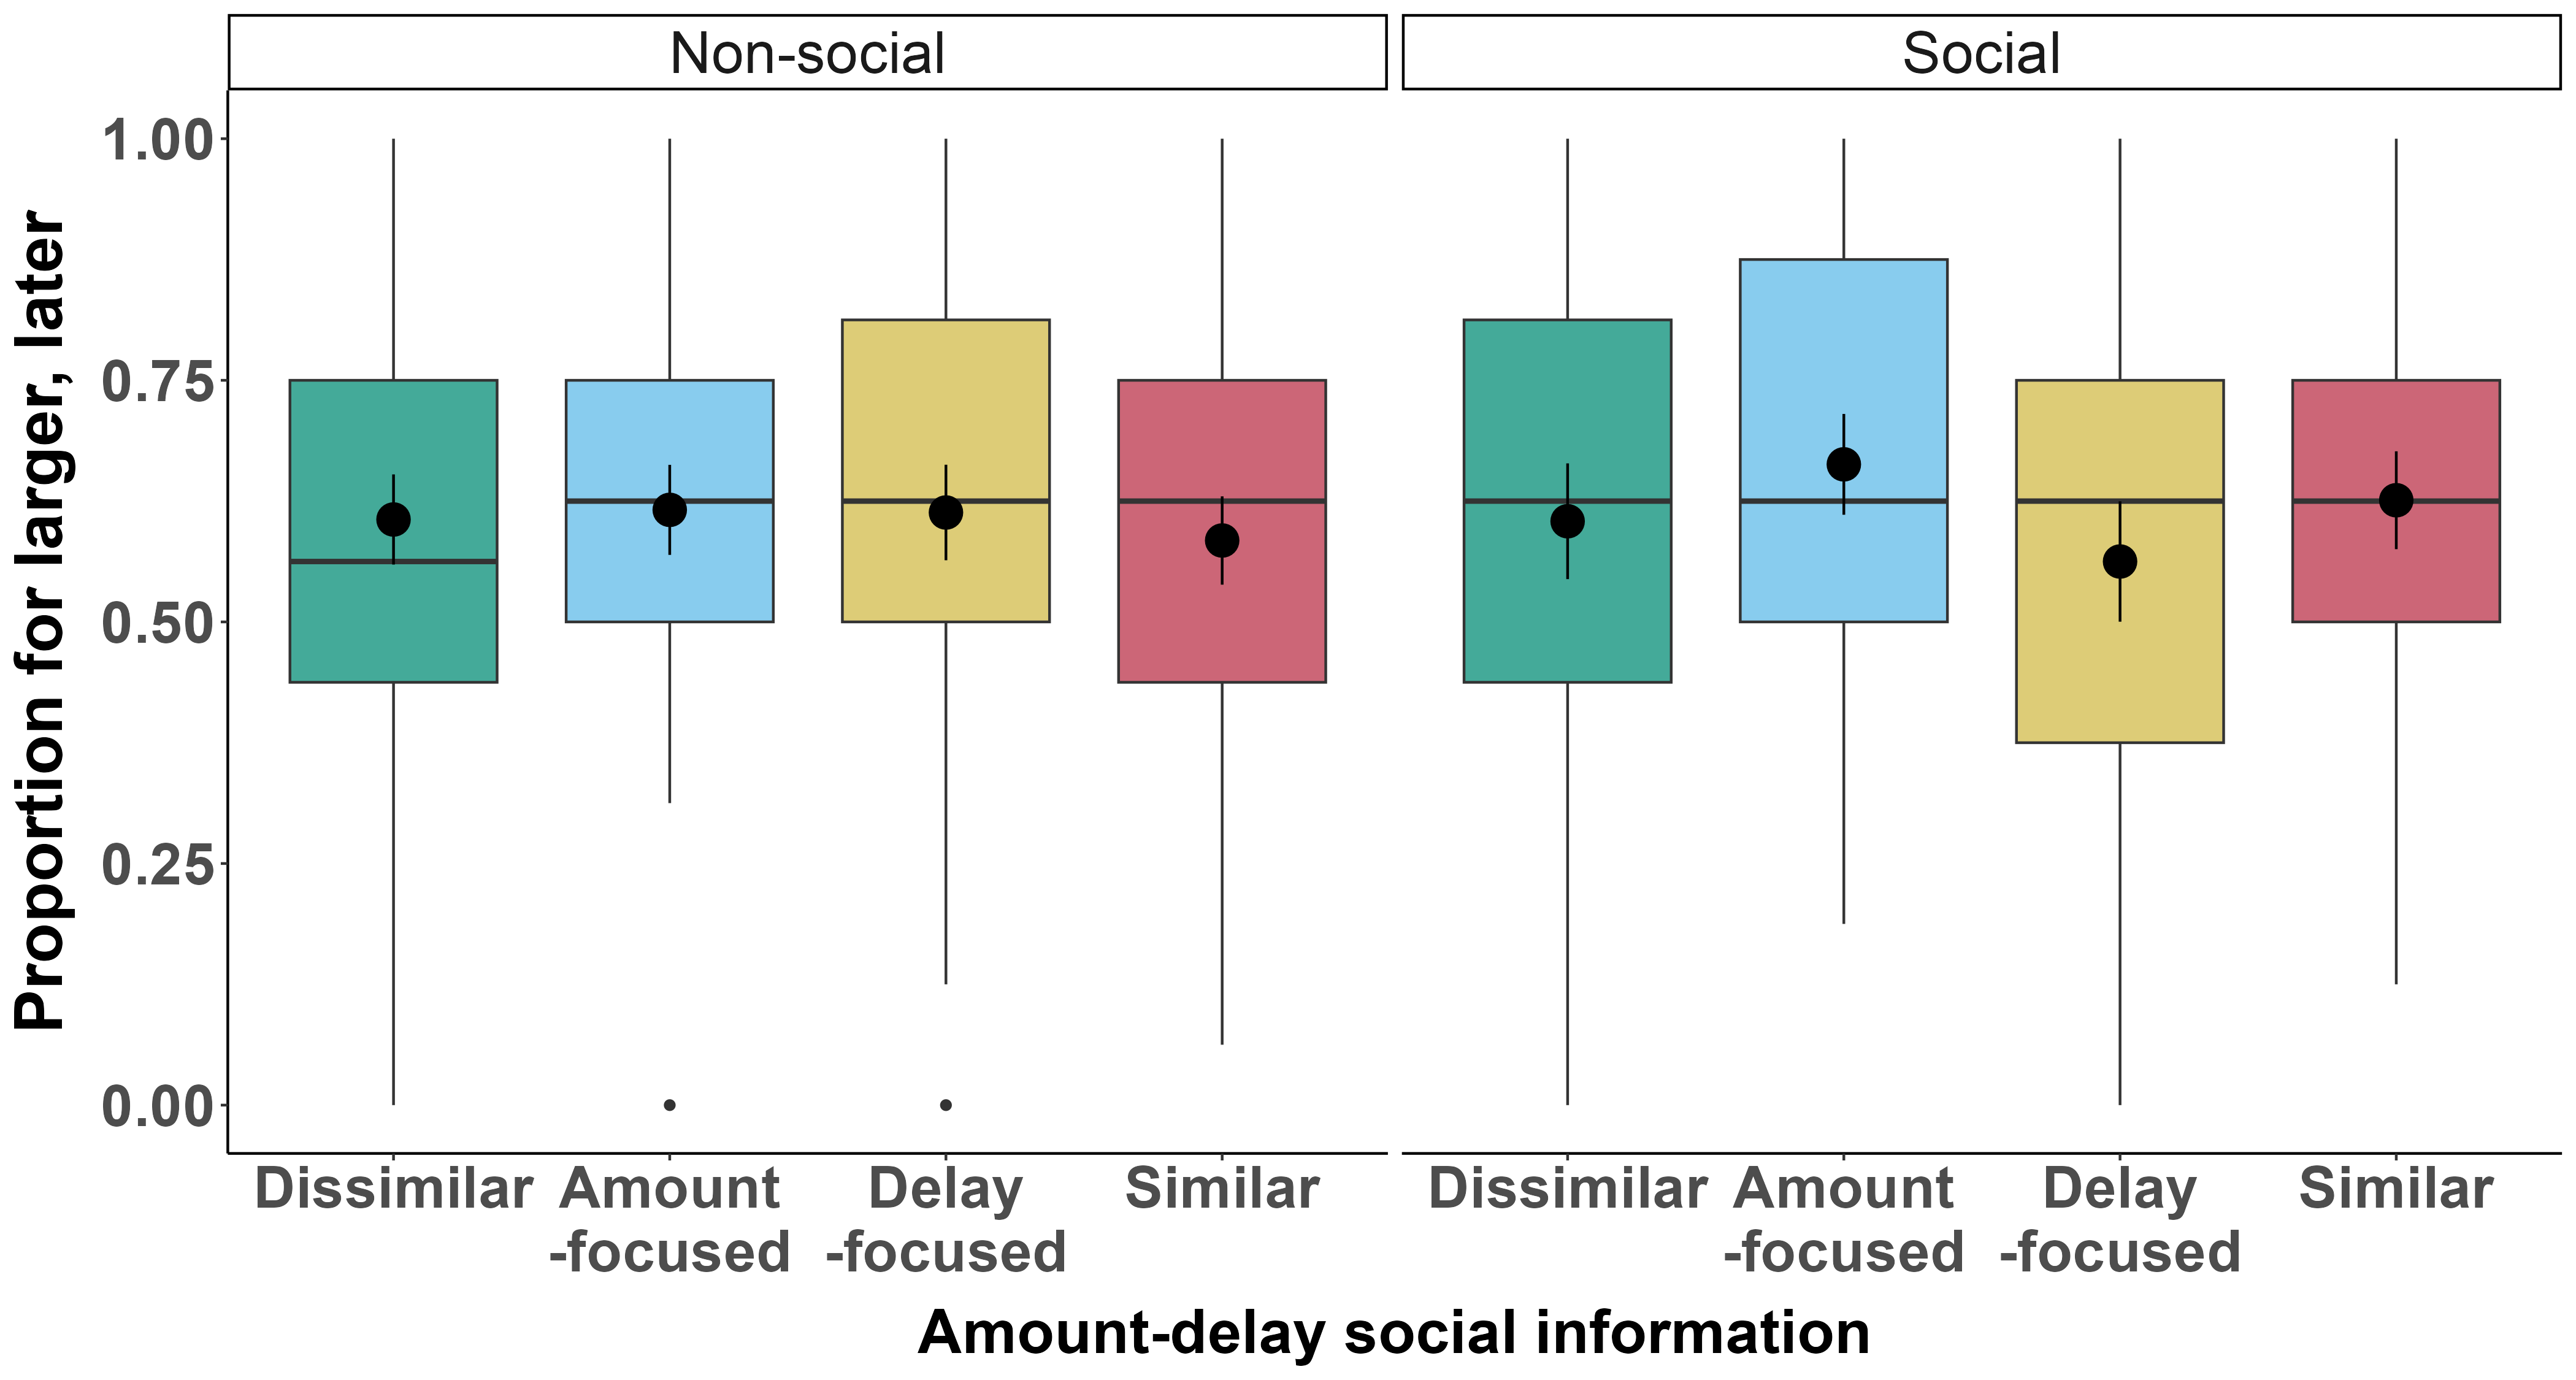
\includegraphics[width=0.8\linewidth]{figures/itc_social_info_1} 

}

\caption{Proportion of participant choices for the larger, later option for non-social (left panel) and social (right panel) intertemporal choice questions across the four social information conditions (dissimilar, amount-focused, delay-focused, and similar) for Study 1. Dots and error bars represent mean values and 95\% within-subject confidence intervals respectively. For boxplots, horizontal bars represent medians, boxes represent interquartile ranges (25\textsuperscript{th} - 75\textsuperscript{th} percentile), and whiskers represent 1.5 times the interquartile range. Figure used with permission under a CC-BY4.0 license: Goh \& Stevens (2022); available at \url{https://doi.org/10.31234/osf.io/xz68b}}\label{fig:socialinfoitc1}
\end{figure*}

To ascertain whether socially suggested information for similarity judgments could shift intertemporal choices, we conducted paired t-tests to compare participant choices across non-social and social intertemporal choice questions for the amount-focused and delay-focused social information conditions. We analyzed the amount-focused and delay-focused social information conditions because they allowed for specific choice predictions to be made using the similarity model. For the amount-focused condition, participants were expected to choose the larger, later option more often for social compared to non-social intertemporal choice questions because they would be making their choices based on the perceived difference between reward amounts. Although participant choices shifted in the predicted direction, the Bayes factor suggested anecdotal evidence for no effect, \(M_D = -0.05\), 95\% CI \([-0.09, 0.00]\), \(t(68) = -2.03\), \(p = .046\), Cohen's \emph{d} = 0.23, \(\mathrm{BF}_{\textrm{10}} = 0.91\). For the delay-focused condition, participants were expected to choose the smaller, sooner option more often for social compared to non-social intertemporal choice questions because they would be making their choices based on the perceived difference between time delays. Though participant choices once again shifted in the predicted direction, the Bayes factor suggested anecdotal evidence for no effect, \(M_D = 0.05\), 95\% CI \([0.00, 0.10]\), \(t(68) = 1.98\), \(p = .051\), Cohen's \emph{d} = 0.22, \(\mathrm{BF}_{\textrm{10}} = 0.83\). However, participant choices for the amount-focused and delay-focused conditions strongly differed when only choices for social intertemporal choice questions were considered (\(M_D = 0.10\), 95\% CI \([0.04, 0.16]\), \(t(68) = 3.19\), \(p = .002\), Cohen's \emph{d} = 0.42, \(\mathrm{BF}_{\textrm{10}} = 12.68\)), suggesting that different social similarity judgments differentially shifted participants' intertemporal choices.

\hypertarget{comparison-of-similarity-judgment-predictions-for-non-social-and-social-intertemporal-choice-questions}{%
\subsubsection{Comparison of similarity judgment predictions for non-social and social intertemporal choice questions}\label{comparison-of-similarity-judgment-predictions-for-non-social-and-social-intertemporal-choice-questions}}

To assess the effect of social information for similarity judgments on intertemporal choice, we compared the accuracy with which participants' personal similarity judgments could predict their choices for non-social and social intertemporal choice questions. That is, we examined the extent to which participants' personal similarity judgments matched the intertemporal choices they were expected to make. Participants were expected to prefer the larger, later option if they indicated amount pairs to be dissimilar in the reward amount similarity judgment task and delay pairs to be similar in the time delay similarity judgment task. When participants initially judged amounts as dissimilar and delays as similar, we found extreme evidence that those judgments predicted both their choices for non-social (\(M = 0.73\), 95\% CI \([0.67, 0.78]\), \(t(61) = 7.80\), \(p < .001\), \(\mathrm{BF}_{\textrm{10}} > 100\)) and social (\(M = 0.69\), 95\% CI \([0.63, 0.75]\), \(t(61) = 6.27\), \(p < .001\), \(\mathrm{BF}_{\textrm{10}} > 100\)) intertemporal choice questions better than chance. The predictive abilities for both types of intertemporal choice questions were not different from each other (\(M_D = 0.03\), 95\% CI \([-0.02, 0.08]\), \(t(61) = 1.33\), \(p = .189\), \(\mathrm{BF}_{\textrm{10}} = 0.32\); Figure \ref{fig:simjudgmentsocialinfopredictions1}a). In contrast, participants were expected to prefer the smaller, sooner option if they indicated amount pairs to be similar in the reward amount similarity judgment task and delay pairs to be dissimilar in the time delay similarity judgment task. However, participants' judgments of similar amounts and dissimilar delays did not predict their choices for non-social intertemporal choice questions (\(M = 0.50\), 95\% CI \([0.44, 0.56]\), \(t(65) = -0.09\), \(p = .928\), \(\mathrm{BF}_{\textrm{10}} = 0.14\)), and there was only anecdotal evidence for effects on social intertemporal choice questions (\(M = 0.42\), 95\% CI \([0.36, 0.49]\), \(t(65) = -2.24\), \(p = .028\), \(\mathrm{BF}_{\textrm{10}} = 1.39\)). We also only found anecdotal evidence that these predictive abilities differed across non-social and social intertemporal choices (\(M_D = 0.07\), 95\% CI \([0.02, 0.13]\), \(t(65) = 2.57\), \(p = .012\), \(\mathrm{BF}_{\textrm{10}} = 2.80\); Figure \ref{fig:simjudgmentsocialinfopredictions1}a). Taken together, these results suggest that similarity judgments predicted intertemporal choices well above chance level---regardless of the presence of social information---when reward amounts were judged dissimilar and time delays were judged similar. However, this predictive ability of similarity judgments for intertemporal choices fell short when reward amounts were judged similar and time delays were judged dissimilar.



\begin{figure*}
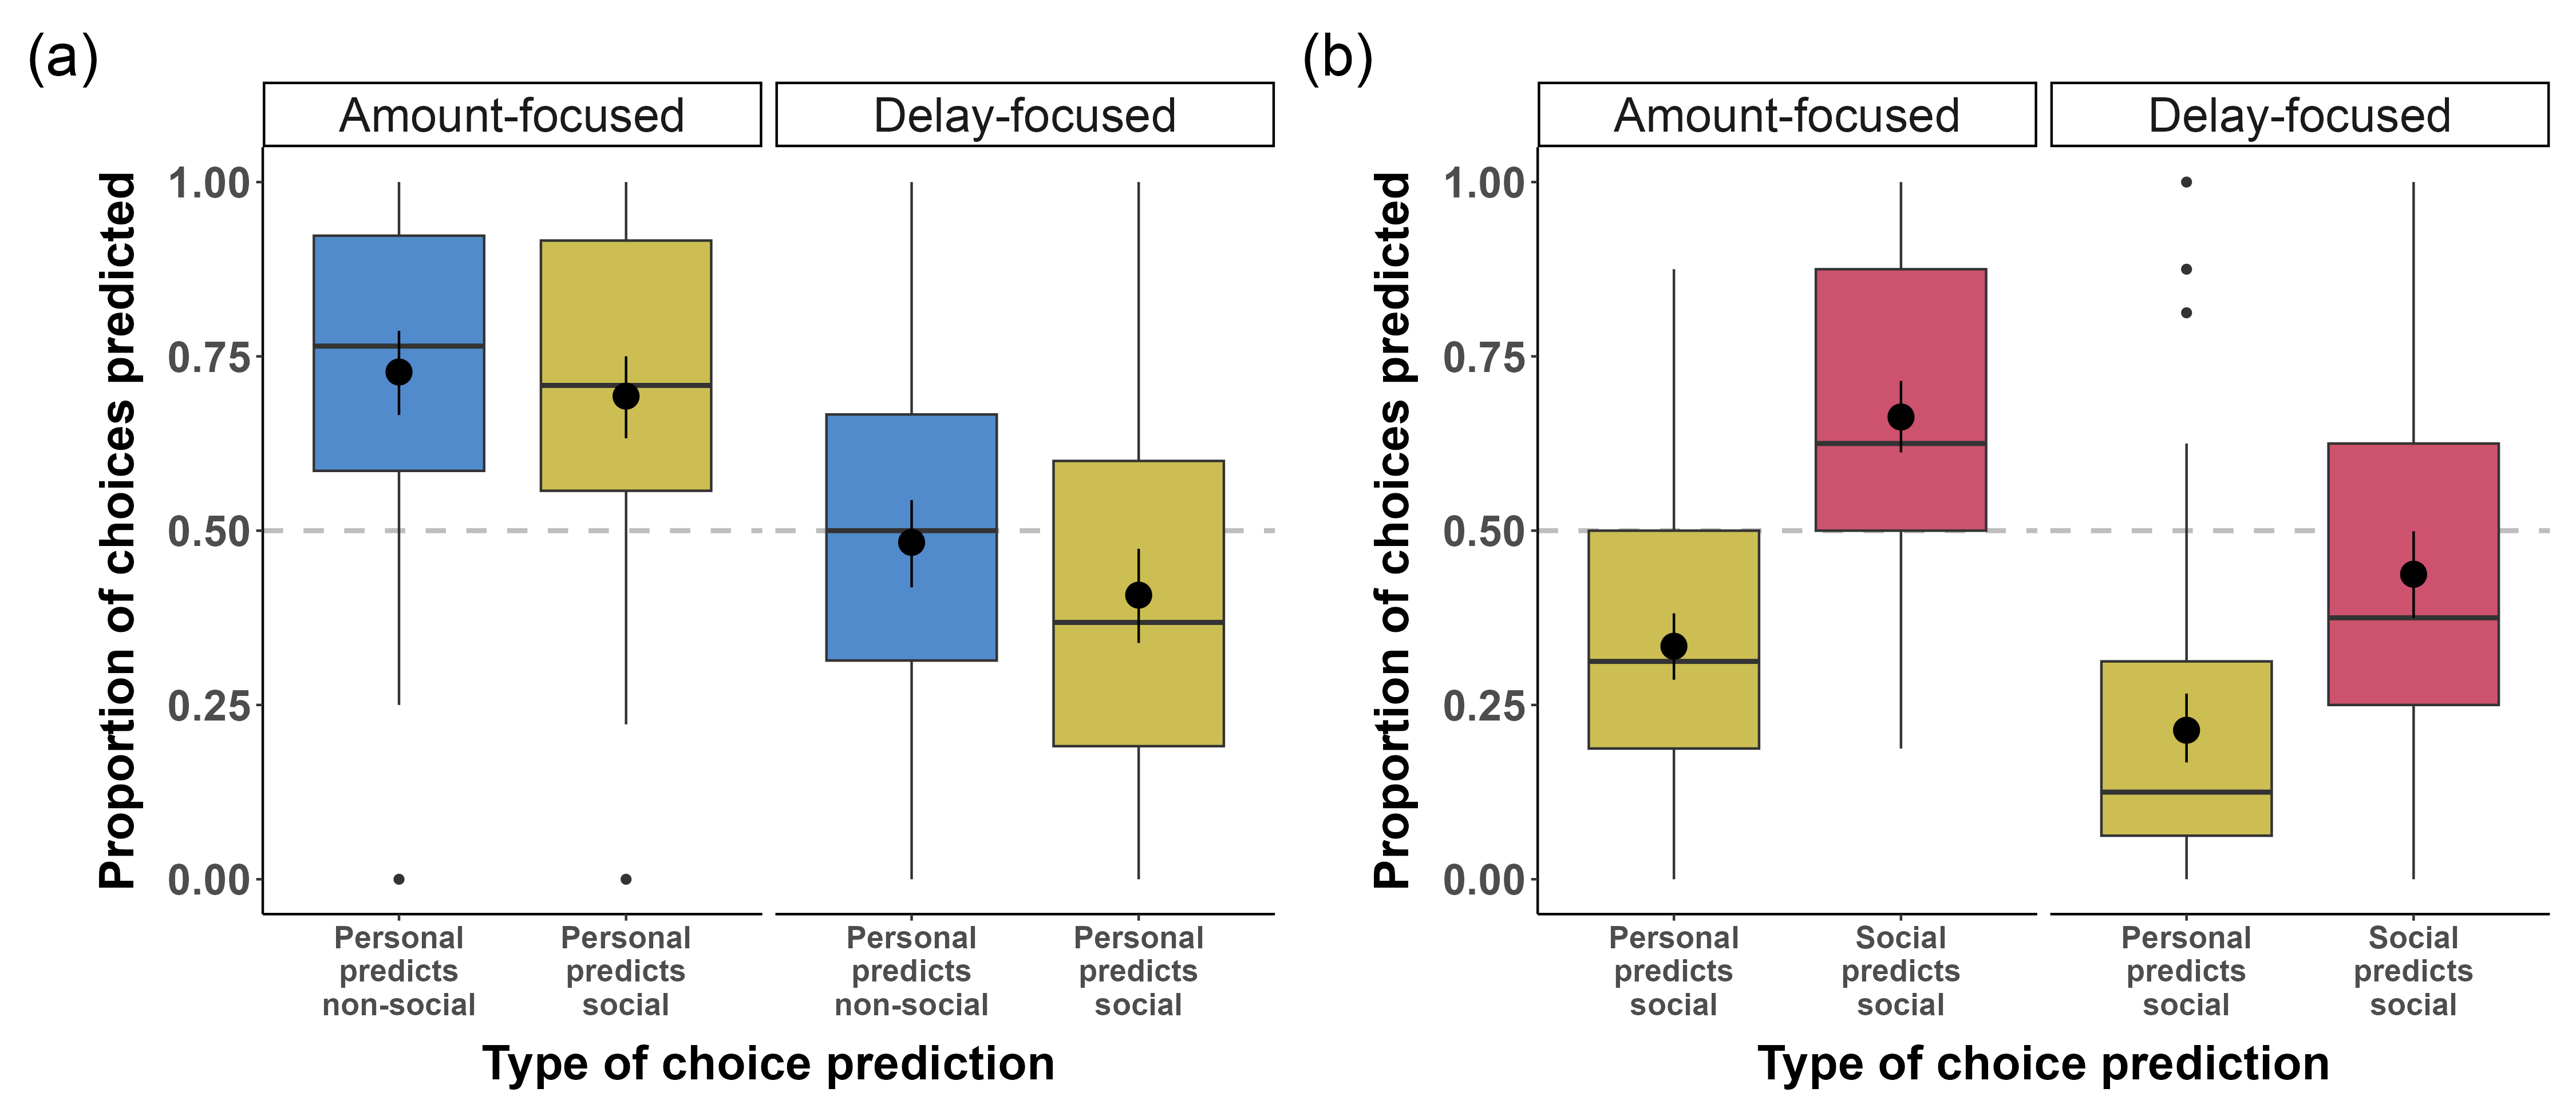
\includegraphics[width=1\linewidth]{figures/sim_judgment_predictions_combined_1} \caption{Proportion of intertemporal choices predicted by participants' reward amount and time delay similarity judgments in the amount-focused (left panels) and delay-focused (right panels) conditions for Study 1. (a) The ``personal predicts non-social'' boxplots represent similarity judgment predictions for non-social intertemporal choice questions while the ``personal predicts social'' boxplots represent similarity judgment predictions for social intertemporal choice questions. (b) The ``personal predicts social'' boxplots represent participants' similarity judgment predictions for social intertemporal choice questions while the ``social predicts social'' boxplots represent presented social information's predictions for social intertemporal choice questions. Dashed lines represent choice predictions at chance (i.e., 50 percent) level, while dots and error bars represent mean values and 95\% within-subject confidence intervals respectively. For boxplots, horizontal bars represent medians, boxes represent interquartile ranges (25\textsuperscript{th} - 75\textsuperscript{th} percentile), and whiskers represent 1.5 times the interquartile range. Figure used with permission under a CC-BY4.0 license: Goh \& Stevens (2022); available at \url{https://doi.org/10.31234/osf.io/xz68b}}\label{fig:simjudgmentsocialinfopredictions1}
\end{figure*}

\hypertarget{comparison-of-similarity-judgment-and-social-information-predictions-for-social-intertemporal-choice-questions}{%
\subsubsection{Comparison of similarity judgment and social information predictions for social intertemporal choice questions}\label{comparison-of-similarity-judgment-and-social-information-predictions-for-social-intertemporal-choice-questions}}

We next compared the accuracy in which participants' similarity judgments and social information could predict their choices for social intertemporal choice questions. That is, we assessed whether their personal judgments or social information about other's judgments best predicted intertemporal choices. For amount-focused questions, results showed extreme evidence that the predictive ability of participants' similarity judgments for social intertemporal choice questions was below chance level (\(M = 0.33\), 95\% CI \([0.29, 0.38]\), \(t(68) = -6.98\), \(p < .001\), \(\mathrm{BF}_{\textrm{10}} > 100\)), whereas the presented social information predicted participants' choices at a better-than-chance level (\(M = 0.66\), 95\% CI \([0.61, 0.72]\), \(t(68) = 6.24\), \(p < .001\), \(\mathrm{BF}_{\textrm{10}} > 100\)). This resulted in a difference in the predictive abilities of both predictors (\(M_D = -0.33\), 95\% CI \([-0.38, -0.28]\), \(t(68) = -12.79\), \(p < .001\), \(\mathrm{BF}_{\textrm{10}} > 100\); Figure \ref{fig:simjudgmentsocialinfopredictions1}b). For delay-focused questions, results showed extreme evidence that participants' similarity judgments did not predict intertemporal choices better than chance (\(M = 0.21\), 95\% CI \([0.16, 0.26]\), \(t(68) = -11.36\), \(p < .001\), \(\mathrm{BF}_{\textrm{10}} > 100\)), with anecdotal evidence that social information predicted choices close to chance level (\(M = 0.44\), 95\% CI \([0.38, 0.50]\), \(t(68) = -2.00\), \(p = .049\), \(\mathrm{BF}_{\textrm{10}} = 0.86\)). However, social information predicted choice better than participants' similarity judgments (\(M_D = -0.22\), 95\% CI \([-0.27, -0.18]\), \(t(68) = -9.22\), \(p < .001\), \(\mathrm{BF}_{\textrm{10}} > 100\); Figure \ref{fig:simjudgmentsocialinfopredictions1}b). Considered together, these results suggest that social information can predict choices for social intertemporal choice questions with greater accuracy compared to participants' similarity judgments across both social information conditions. However, social information only predicted choices above chance level for amount-focused questions.

\hypertarget{suggestibility-effects-on-social-influence}{%
\subsubsection{Suggestibility effects on social influence}\label{suggestibility-effects-on-social-influence}}

To test the effect of suggestibility on social influence, we compared participants' responses for the amount-focused and delay-focused social information conditions by suggestibility level. For the amount-focused condition, participants in the high suggestibility group were expected to choose the larger, later option in social intertemporal choice questions (compared to non-social intertemporal choice questions) more often than participants in the low suggestibility group. Though the frequentist analysis of the results showed a shift from smaller, sooner to larger, later intertemporal choice options between the two suggestibility groups (\(F(1, 67) = 5.26\), \(p = .025\), \(\hat{\eta}^2_G = .016\), 90\% CI \([.000, .098]\), \(\mathrm{BF}_{\textrm{10}} = 0.70\)), the Bayes factor suggested anecdotal evidence that did not support this finding (Figure S1a). A post-hoc test using Tukey's HSD revealed that participants in the high suggestibility group chose the larger, later option more often in social compared to non-social intertemporal choice questions as predicted (\(\Delta M = -0.09\), 95\% CI \([-0.15, -0.03]\), \(t(67) = -3.09\), \(p = .003\)). In contrast, a pairwise comparison for participants in the low suggestibility group suggested that they did not choose the larger, later option more often in social compared to non-social intertemporal choice questions (\(\Delta M = 0.01\), 95\% CI \([-0.06, 0.08]\), \(t(67) = 0.30\), \(p = .765\)).

For the delay-focused condition, participants in the high suggestibility group were expected to choose the smaller, sooner option in social intertemporal choice questions (compared to non-social intertemporal choice questions) more often than participants in the low suggestibility group. Results yielded moderate evidence for no difference in shifts from larger, later to smaller, sooner intertemporal choices between the two suggestibility groups (\(F(1, 67) = 0.00\), \(p = .991\), \(\hat{\eta}^2_G = .000\), 90\% CI \([.000, .000]\), \(\mathrm{BF}_{\textrm{10}} = 0.27\); Figure S1b). Collectively, while the shifts in participant choices across intertemporal choice questions seem to suggest that suggestibility affects social information effects on similarity judgments and subsequent intertemporal choices when the larger, later option is the socially suggested option, more evidence is required to support this conclusion.

\hypertarget{numeracy-effects-on-similarity-judgments-and-intertemporal-choices}{%
\subsubsection{Numeracy effects on similarity judgments and intertemporal choices}\label{numeracy-effects-on-similarity-judgments-and-intertemporal-choices}}

Participants with higher objective and subjective numeracy scores were expected to judge a lower proportion of number pairs in each similarity judgment task as similar compared to participants with lower scores. In terms of objective numeracy, participants did not differ in similarity judgments based on their objective numeracy scores for both amount (\(\chi\)\textsuperscript{2}(1) = 0.01, \emph{p} = .929, \(\mathrm{BF}_{\textrm{10}} = 0.02\)) and delay (\(\chi\)\textsuperscript{2}(1) = 0.44, \emph{p} = .508, \(\mathrm{BF}_{\textrm{10}} = 0.02\)) similarity judgment tasks (Figure S2a). Similarly, in terms of subjective numeracy, participants high in subjective numeracy did not judge number pairs as less similar compared to those low in subjective numeracy for both amount (\(\chi\)\textsuperscript{2}(1) = 0.41, \emph{p} = .524, \(\mathrm{BF}_{\textrm{10}} = 0.02\)) and delay (\(\chi\)\textsuperscript{2}(1) = 0.83, \emph{p} = .362, \(\mathrm{BF}_{\textrm{10}} = 0.03\)) similarity judgments tasks (Figure S2b). Contrary to our prediction that individuals with higher numeracy would judge values in number pairs as less similar compared to those with lower numeracy, our results showed that numeracy did not affect similarity judgments.

Besides testing for differences in similarity judgments for reward amounts and time delays, we tested participant preferences for the larger, later option in non-social intertemporal choice questions according to numeracy. Participants with higher numeracy were predicted to prefer the larger, later option more often in non-social intertemporal choice questions compared to participants with lower numeracy because highly numerate individuals should be less influenced by option framing effects and therefore prefer the option with the greater reward amount (Cokely et al., 2012; Peters, 2012; Ghazal et al., 2014). Participants with higher numeracy scores did not choose the larger, later option more often compared to participants with lower scores for both objective numeracy (\(\chi\)\textsuperscript{2}(1) = 0.13, \emph{p} = .716, \(\mathrm{BF}_{\textrm{10}} = 0.02\); Figure S3a) and subjective numeracy (\(\chi\)\textsuperscript{2}(1) = 0.00, \emph{p} = .955, \(\mathrm{BF}_{\textrm{10}} = 0.02\); Figure S3b). Thus, participants with higher numeracy did not prefer the larger, later option in intertemporal choice questions more often than those with lower numeracy.

\hypertarget{discussion}{%
\subsection{\texorpdfstring{\emph{Discussion}}{Discussion}}\label{discussion}}

The present study offers preliminary evidence that social information can affect intertemporal choice by shifting similarity judgments, suggesting support for Hypothesis 1. Specifically, participants' intertemporal choices varied when they viewed different social information that presented similarity judgments for reward amounts and time delays. Follow-up analyses revealed that participants' personal similarity judgments predicted their choices for non-social and social intertemporal choice questions at better than chance levels when they judged amounts to be dissimilar and delays to be similar, but not when they judged amounts to be similar and delays to be dissimilar. In contrast, social information predicted participants' choices for social intertemporal choice questions at greater than chance levels only when participants viewed social information that suggested amounts to be dissimilar and delays to be similar. Further, suggestibility may moderate the effect of social information on intertemporal choice when the larger, later option is the socially suggested option, suggesting partial support for Hypothesis 2. Finally, numeracy affected neither participants' similarity judgments nor intertemporal choices, suggesting no support for Hypothesis 3.

A limitation of the present study was the high attrition rate that greatly reduced the participant sample size. This resulted in only anecdotal evidence for some analyses, which suggested a need for more evidence to distinguish between hypotheses. The repetitive nature of the similarity judgment and intertemporal choice questions, coupled with the large number of questions for each task could have led participants to lose interest in the study as it progressed, thus increasing the probability of them failing attention check questions and the likelihood of making intertemporal choices at random so they could complete the study quickly.

\hypertarget{study-2-replication}{%
\section{Study 2: Replication}\label{study-2-replication}}

The aim of the present study was to replicate the findings from Study 1 using a reduced number of intertemporal choice questions so that more specific conclusions could be reached on how social information affects intertemporal choice. To achieve this, we used only questions from the two social information conditions that allowed for intertemporal choice predictions to be made (i.e., the delay-focused and amount-focused social information conditions).

\hypertarget{methods-1}{%
\subsection{\texorpdfstring{\emph{Methods}}{Methods}}\label{methods-1}}

\hypertarget{participants-and-procedures-1}{%
\subsubsection{Participants and procedures}\label{participants-and-procedures-1}}

Participants were 86 undergraduates (63 women, 22 men, 1 unspecified; M\textsubscript{age} = 19.38, SD = 1.40) recruited from the undergraduate psychology study pool at the University of Nebraska-Lincoln who participated for course research credit from February to October 2019. The majority of participants were white (77\%; see Table S1 for detailed description). Data from an additional 67 participants were excluded from analyses because these participants either failed attention check questions that were embedded throughout the study or had nearly exclusive preferences for one option for similarity judgment and intertemporal choice questions.

The procedure for the present study was identical to that of Study 1 with the exception of a reduced number of social intertemporal choice questions in the intertemporal choice phase. Like Study 1, participants viewed the same number of social intertemporal choice questions that stated (1) reward amounts were judged dissimilar but time delays were judged similar (amount-focused condition), and (2) reward amounts were judged similar but time delays were judged dissimilar (delay-focused condition). Unlike Study 1, participants viewed only four questions that stated either both reward amounts and time delays were judged similar or both reward amounts and time delays were judged dissimilar because these questions merely served as distractors in the present study.

\hypertarget{data-analysis-1}{%
\subsubsection{Data analysis}\label{data-analysis-1}}

The present study was pre-registered at AsPredicted.org before data collection (\url{https://aspredicted.org/blind.php?x=ge9if5}). Analyses for the effects of social information on intertemporal choice, and suggestibility and numeracy effects on social influence were the same as those for Study 1.

\hypertarget{results-1}{%
\subsection{\texorpdfstring{\emph{Results}}{Results}}\label{results-1}}

\hypertarget{effect-of-social-information-on-intertemporal-choices-1}{%
\subsubsection{Effect of social information on intertemporal choices}\label{effect-of-social-information-on-intertemporal-choices-1}}

Results of our 2x2 repeated-measures ANOVA revealed moderate and anecdotal evidence for no main effect for intertemporal choice question type (\(F(1, 85) = 1.92\), \(p = .170\), \(\hat{\eta}^2_G = .002\), 90\% CI \([.000, .042]\), \(\mathrm{BF}_{\textrm{10}} = 0.26\)) or social information condition on intertemporal choices (\(F(1, 85) = 3.89\), \(p = .052\), \(\hat{\eta}^2_G = .004\), 90\% CI \([.000, .055]\), \(\mathrm{BF}_{\textrm{10}} = 0.88\)) respectively. There was strong evidence for an interaction effect between intertemporal choice question type and social information condition on intertemporal choice (\(F(1, 85) = 11.06\), \(p = .001\), \(\hat{\eta}^2_G = .010\), 90\% CI \([.000, .073]\), \(\mathrm{BF}_{\textrm{10}} = 22.37\); Figure \ref{fig:socialinfoitccomparison2}). A post-hoc test using Tukey's HSD showed that participants chose the larger, later option more often in the amount-focused condition for social intertemporal choice questions (\(\Delta M = -0.06\), 95\% CI \([-0.09, -0.03]\), \(t(85) = -3.58\), \(p = .001\)).

We next conducted paired t-tests to compare participant choices across the amount-focused and delay-focused conditions of the non-social and social intertemporal choice tasks. For the amount-focused condition, there was very strong evidence that participants chose the larger, later option more often for social compared to non-social intertemporal choice questions (\(M_D = -0.06\), 95\% CI \([-0.09, -0.03]\), \(t(85) = -3.58\), \(p = .001\), Cohen's \emph{d} = 0.29, \(\mathrm{BF}_{\textrm{10}} = 39.47\)). For the delay-focused condition, there was moderate evidence that participants did not choose the smaller, sooner option more often for social compared to non-social intertemporal choice questions (\(M_D = 0.03\), 95\% CI \([-0.01, 0.06]\), \(t(85) = 1.35\), \(p = .180\), Cohen's \emph{d} = 0.12, \(\mathrm{BF}_{\textrm{10}} = 0.29\)). However, participant choices for the amount-focused and delay-focused conditions strongly differed when only choices for social intertemporal choice questions were considered (\(M_D = 0.07\), 95\% CI \([0.03, 0.11]\), \(t(85) = 3.16\), \(p = .002\), Cohen's \emph{d} = 0.32, \(\mathrm{BF}_{\textrm{10}} = 11.71\)), suggesting that opposing social similarity judgments differentially shifted participants' intertemporal choices.



\begin{figure}
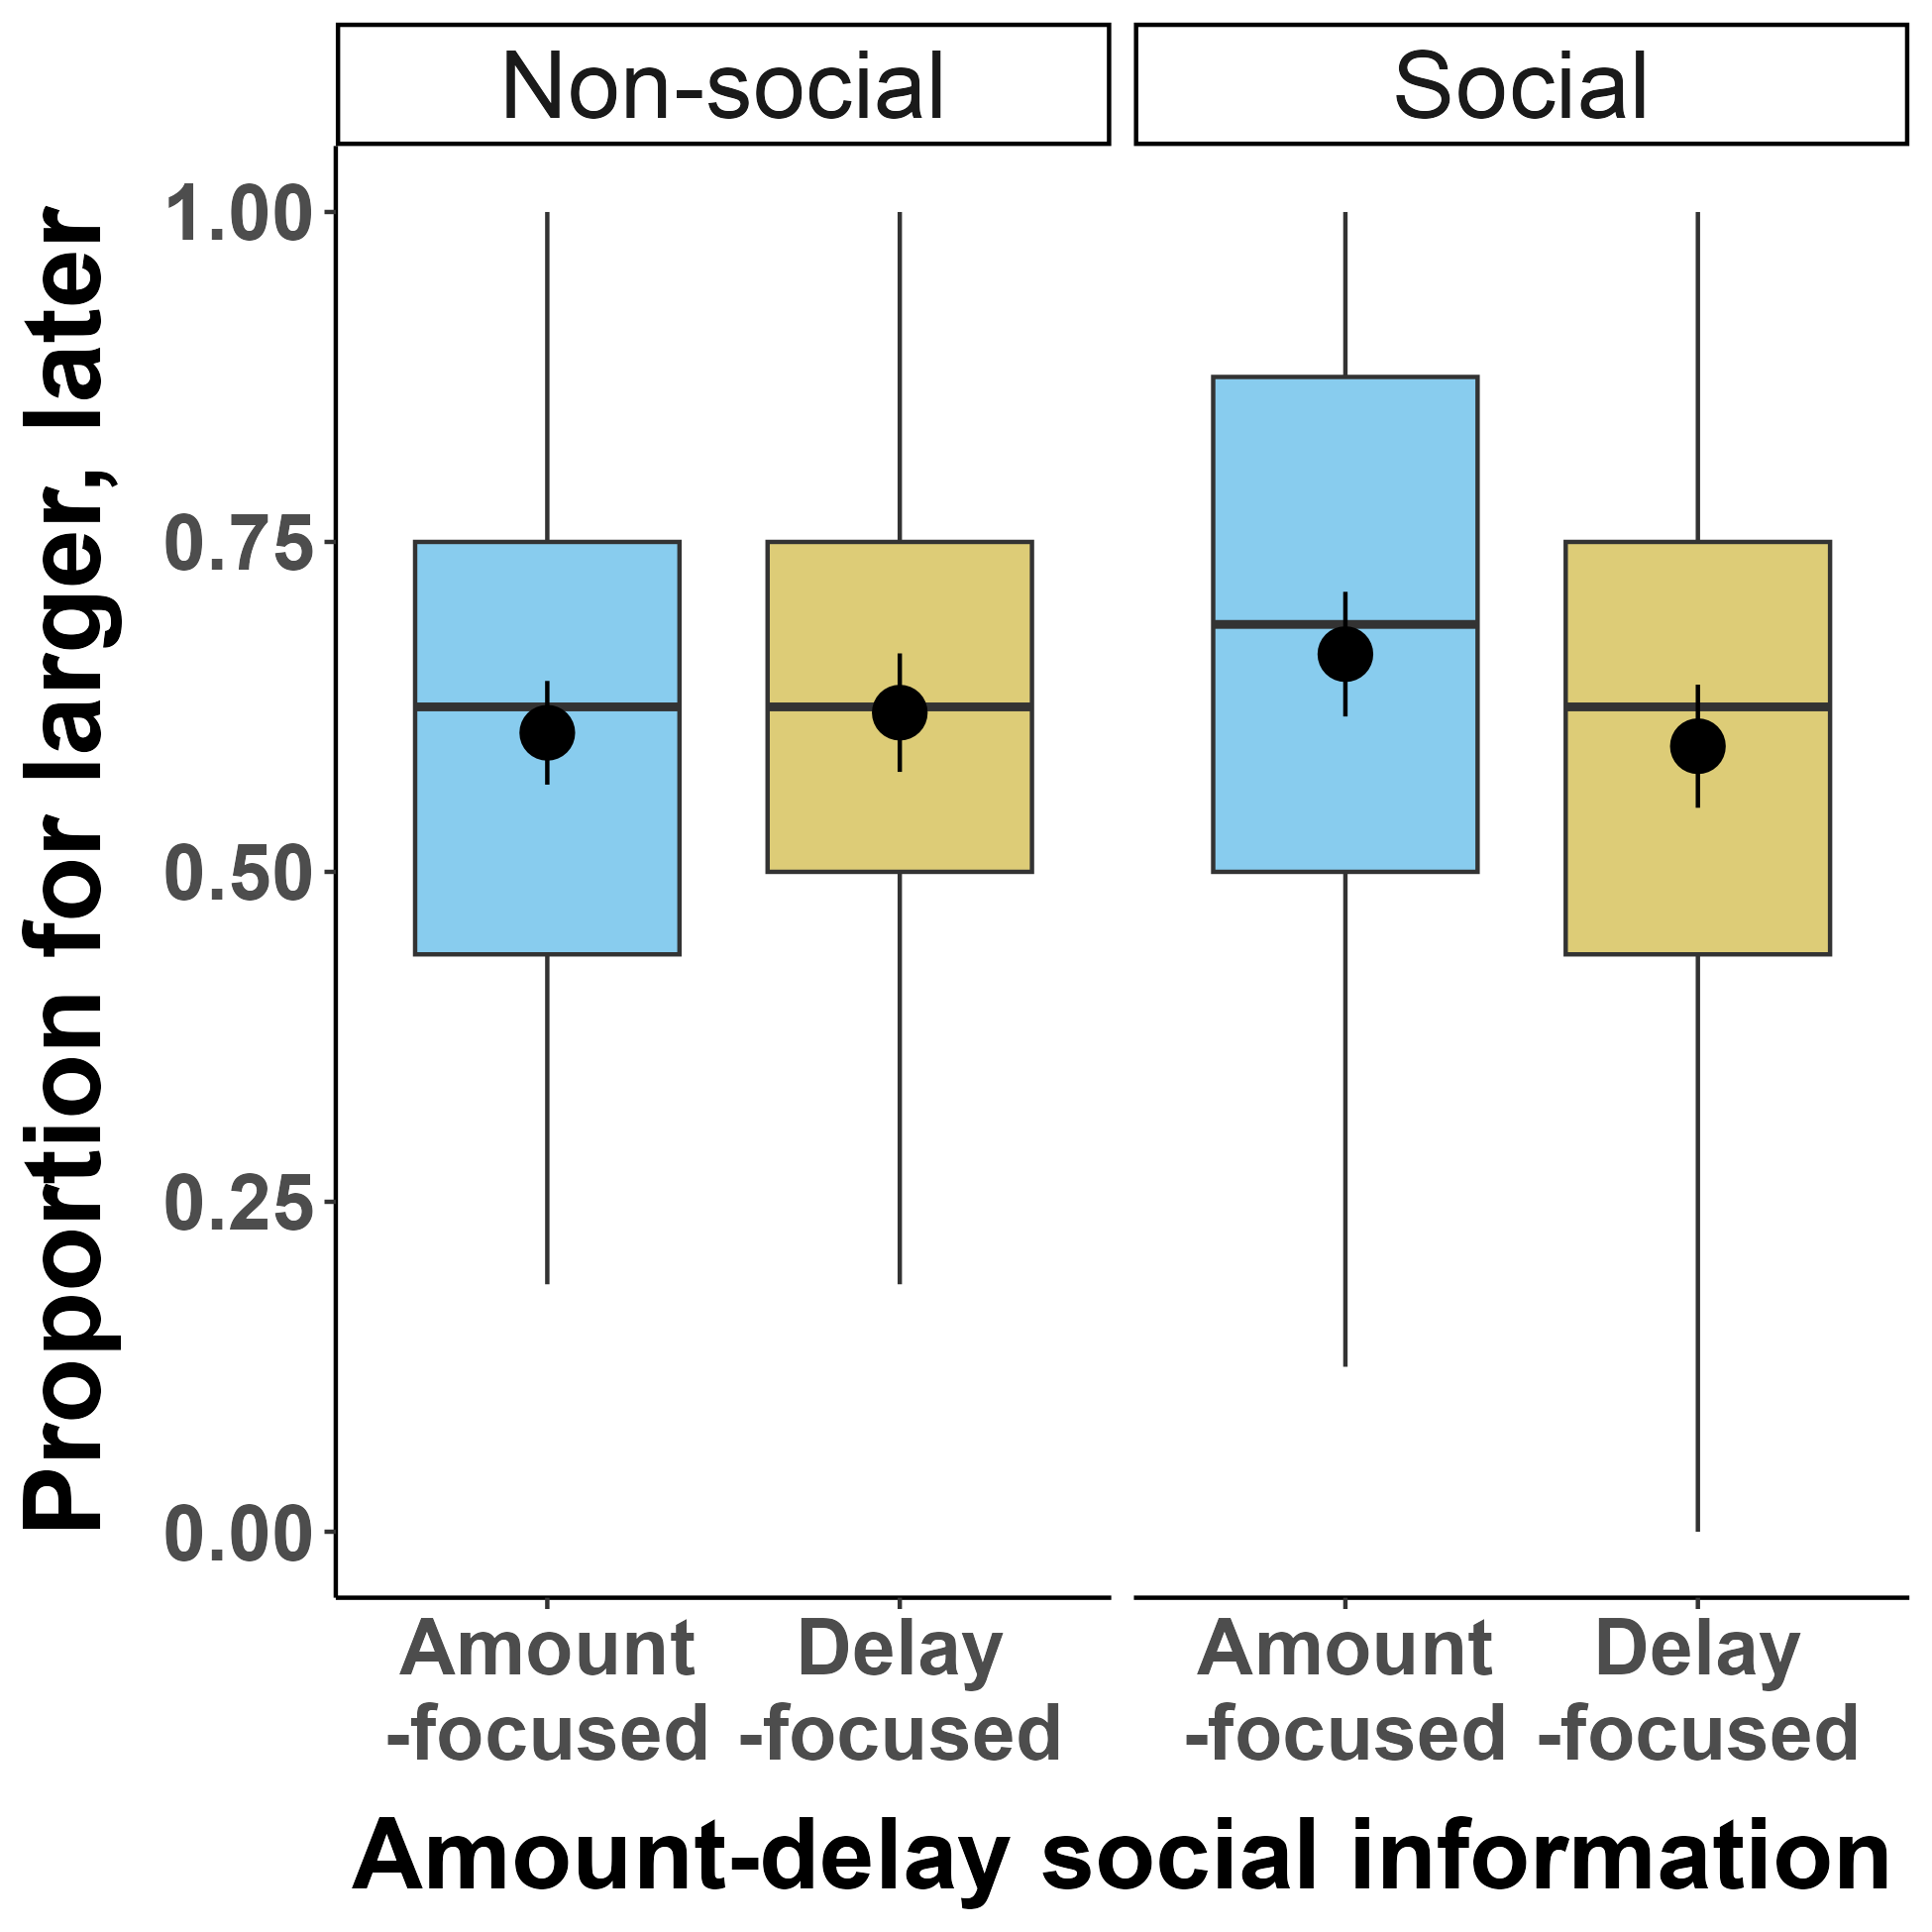
\includegraphics[width=1\linewidth]{figures/itc_social_info_2} \caption{Proportion of participant choices for the larger, later option for non-social (left panel) and social (right panel) intertemporal choice questions for the amount-focused and delay-focused social information conditions for Study 2. Dots and error bars represent mean values and 95\% within-subject confidence intervals respectively. Boxplots show the range of values and values at the 25th percentile, 50th percentile (median) and 75th percentile. Figure used with permission under a CC-BY4.0 license: Goh \& Stevens (2022); available at \url{https://doi.org/10.31234/osf.io/xz68b}}\label{fig:socialinfoitccomparison2}
\end{figure}

\hypertarget{comparison-of-similarity-judgment-predictions-for-non-social-and-social-intertemporal-choice-questions-1}{%
\subsubsection{Comparison of similarity judgment predictions for non-social and social intertemporal choice questions}\label{comparison-of-similarity-judgment-predictions-for-non-social-and-social-intertemporal-choice-questions-1}}

Participants were expected to prefer the larger, later option if they indicated amount pairs to be dissimilar in the reward amount similarity judgment task and delay pairs to be similar in the time delay similarity judgment task (amount-focused condition). There was extreme evidence that participants' similarity judgments predicted both their choices for non-social (\(M = 0.73\), 95\% CI \([0.67, 0.78]\), \(t(76) = 8.25\), \(p < .001\), \(\mathrm{BF}_{\textrm{10}} > 100\)) and social (\(M = 0.76\), 95\% CI \([0.71, 0.81]\), \(t(76) = 10.52\), \(p < .001\), \(\mathrm{BF}_{\textrm{10}} > 100\)) intertemporal choice questions above chance level, and moderate evidence that the predictive abilities for both types of questions did not differ from each other (\(M_D = -0.03\), 95\% CI \([-0.08, 0.02]\), \(t(76) = -1.15\), \(p = .252\), \(\mathrm{BF}_{\textrm{10}} = 0.24\); Figure \ref{fig:simjudgmentsocialinfopredictions2}a). In contrast, participants were expected to prefer the smaller, sooner option if they indicated amount pairs to be similar in the reward amount similarity judgment task and delay pairs to be dissimilar in the time delay similarity judgment task (delay-focused condition). Results yielded moderate evidence that participants' similarity judgments did not predict choices for non-social intertemporal choice questions (\(M = 0.51\), 95\% CI \([0.45, 0.57]\), \(t(79) = 0.29\), \(p = .770\), \(\mathrm{BF}_{\textrm{10}} = 0.13\)) and anecdotal evidence that similarity judgments did not predict social intertemporal choice questions (\(M = 0.45\), 95\% CI \([0.38, 0.52]\), \(t(79) = -1.51\), \(p = .135\), \(\mathrm{BF}_{\textrm{10}} = 0.37\)) above chance level. However, there was anecdotal evidence that participants' similarity judgments better predicted their choices for non-social compared to social intertemporal choice questions (\(M_D = 0.06\), 95\% CI \([0.00, 0.12]\), \(t(79) = 2.07\), \(p = .042\), \(\mathrm{BF}_{\textrm{10}} = 0.92\); Figure \ref{fig:simjudgmentsocialinfopredictions2}a). Collectively, these results replicate those of Study 1 where similarity judgments predicted intertemporal choices well above chance level in the amount-focused condition (i.e., when reward amounts are judged dissimilar and time delays are judged similar), but not in the delay-focused condition (i.e., when reward amounts are judged similar and time delays are judged dissimilar).

\hypertarget{comparison-of-similarity-judgment-and-social-information-predictions-for-social-intertemporal-choice-questions-1}{%
\subsubsection{Comparison of similarity judgment and social information predictions for social intertemporal choice questions}\label{comparison-of-similarity-judgment-and-social-information-predictions-for-social-intertemporal-choice-questions-1}}

Social information was expected to predict participants' preferences for larger, later options for amount-focused social intertemporal choice questions. Results showed extreme evidence that the predictive ability of participants' similarity judgments for social intertemporal choice questions was below chance level (\(M = 0.37\), 95\% CI \([0.32, 0.42]\), \(t(85) = -5.63\), \(p < .001\), \(\mathrm{BF}_{\textrm{10}} > 100\)) and extreme evidence that the presented social information predicted participants' choices at above chance level (\(M = 0.66\), 95\% CI \([0.62, 0.71]\), \(t(85) = 6.95\), \(p < .001\), \(\mathrm{BF}_{\textrm{10}} > 100\)). This resulted in a difference in the predictive abilities of both predictors (\(M_D = -0.29\), 95\% CI \([-0.34, -0.25]\), \(t(85) = -12.25\), \(p < .001\), \(\mathrm{BF}_{\textrm{10}} > 100\); Figure \ref{fig:simjudgmentsocialinfopredictions2}b).

In contrast, social information was expected to predict participants' preferences for smaller, sooner options for delay-focused social intertemporal choice questions. Results showed extreme evidence that neither participants' similarity judgments (\(M = 0.25\), 95\% CI \([0.21, 0.28]\), \(t(85) = -14.54\), \(p < .001\), \(\mathrm{BF}_{\textrm{10}} > 100\)) nor presented social information (\(M = 0.40\), 95\% CI \([0.36, 0.45]\), \(t(85) = -4.06\), \(p < .001\), \(\mathrm{BF}_{\textrm{10}} > 100\)) predicted choices for social intertemporal choice questions better than chance though there was extreme evidence that social information was a better predictor than participants' similarity judgments (\(M_D = -0.16\), 95\% CI \([-0.19, -0.13]\), \(t(85) = -9.91\), \(p < .001\), \(\mathrm{BF}_{\textrm{10}} > 100\); Figure \ref{fig:simjudgmentsocialinfopredictions2}b). Together, these results replicate those of Study 1 where social information predicted intertemporal choices at better than chance level when reward amounts were suggested to be dissimilar and time delays similar, and that social information better predicted social intertemporal choices compared to participants' personal similarity judgments.



\begin{figure*}
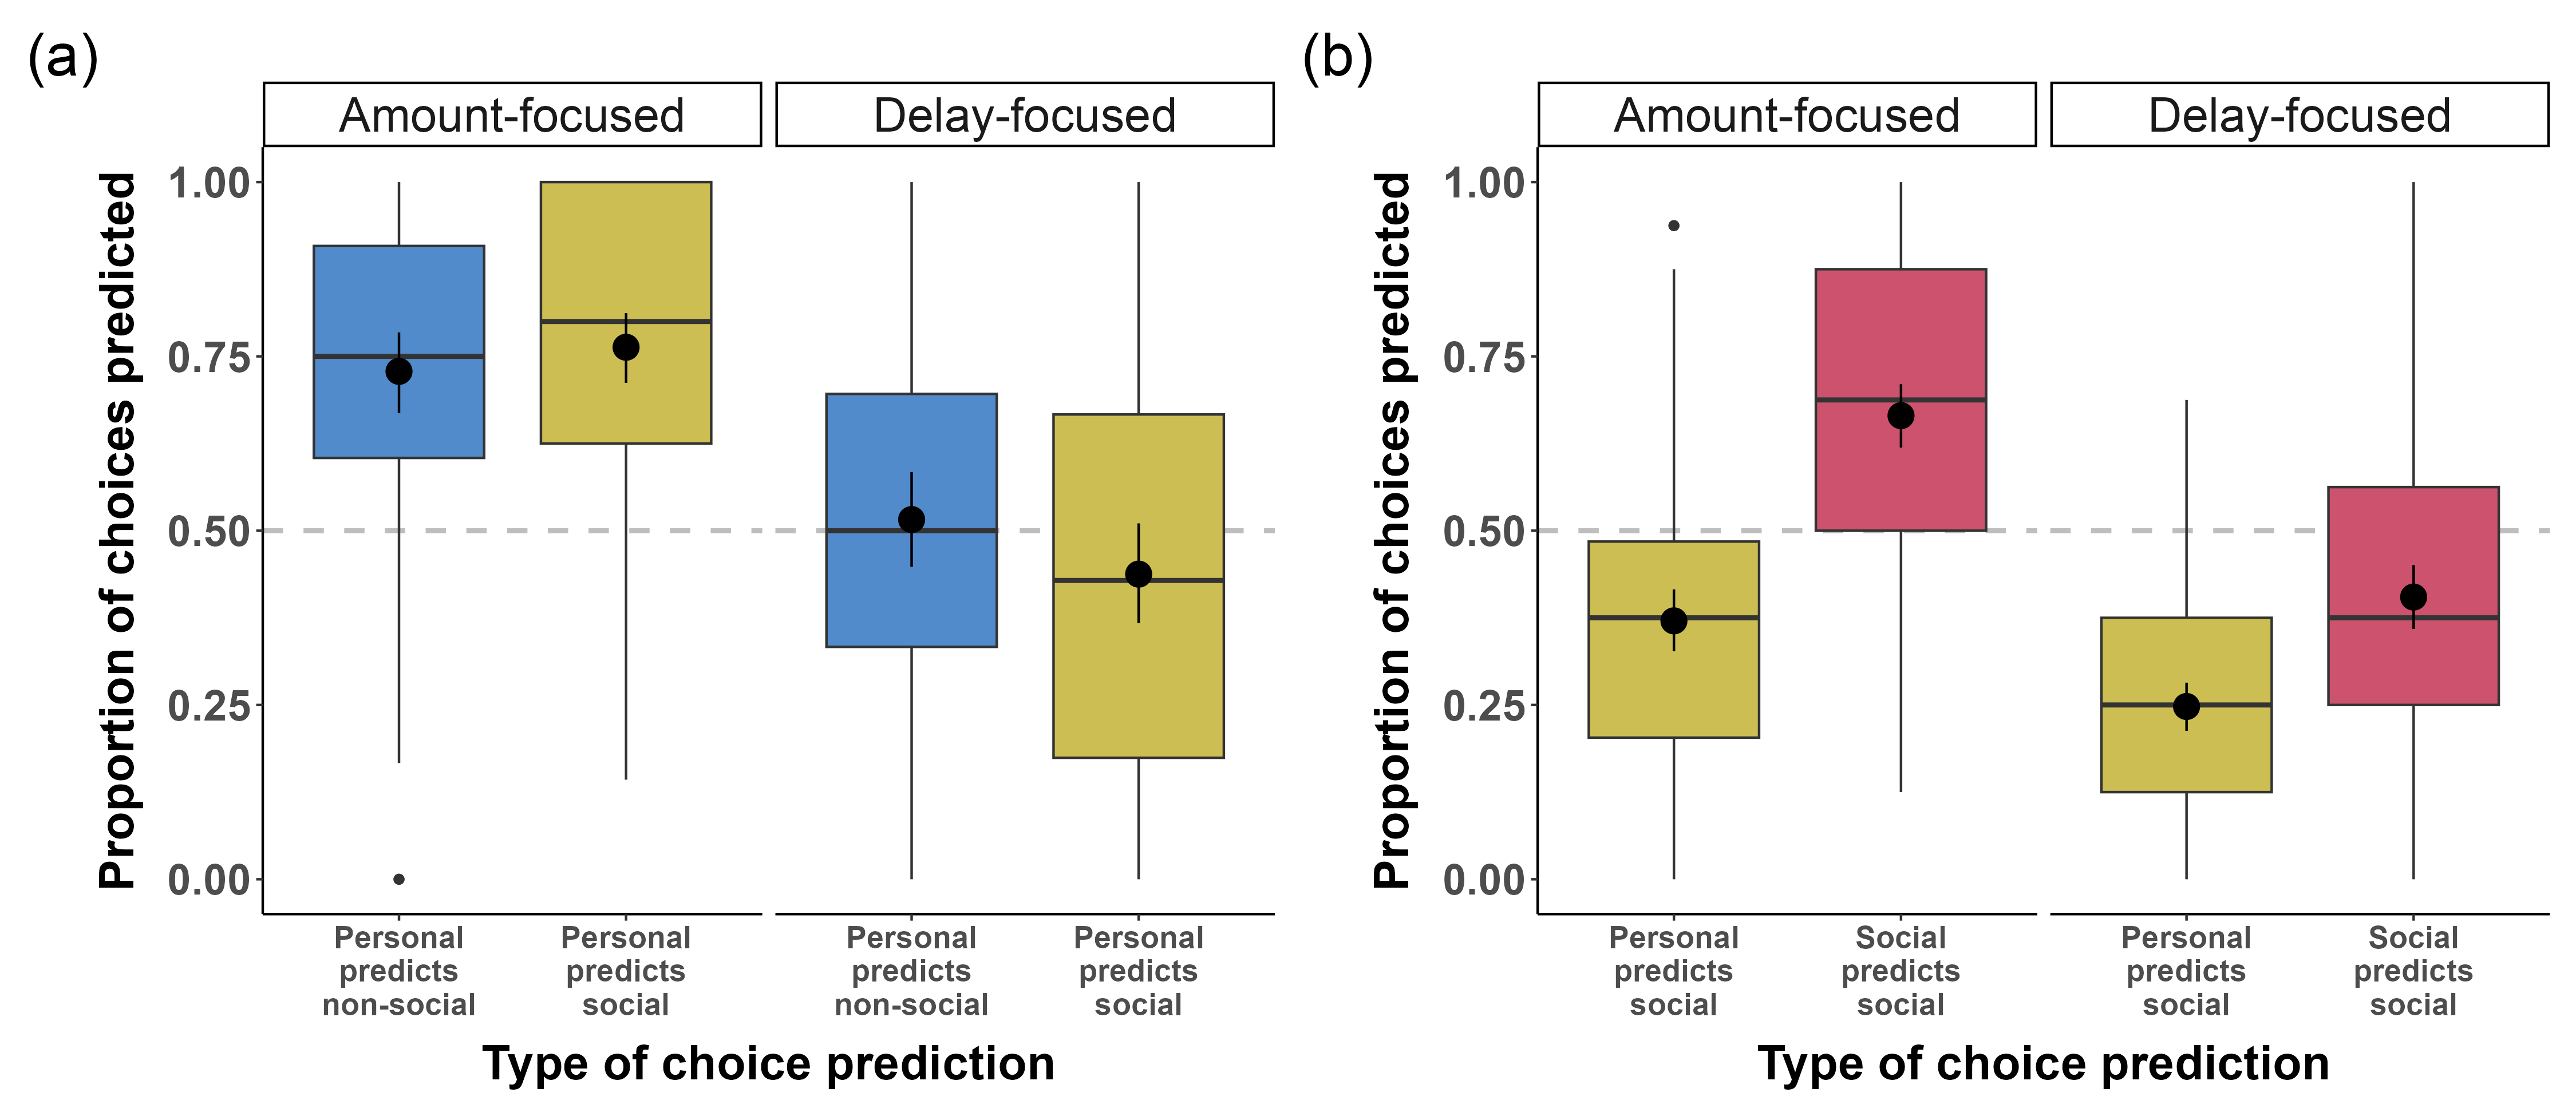
\includegraphics[width=1\linewidth]{figures/sim_judgment_predictions_combined_2} \caption{Proportion of intertemporal choices predicted by participants' reward amount and time delay similarity judgments in the amount-focused (left panels) and delay-focused (right panels) conditions for Study 2. (a) The ``personal predicts non-social'' boxplots represent similarity judgment predictions for non-social intertemporal choice questions while the ``personal predicts social'' boxplots represent similarity judgment predictions for social intertemporal choice questions. (b) The ``personal predicts social'' boxplots represent participants' similarity judgment predictions for social intertemporal choice questions while the ``social predicts social'' boxplots represent presented social information's predictions for social intertemporal choice questions. Dashed lines represent choice predictions at chance (i.e., 50 percent) level, while dots and error bars represent mean values and 95\% within-subject confidence intervals respectively. For boxplots, horizontal bars represent medians, boxes represent interquartile ranges (25\textsuperscript{th} - 75\textsuperscript{th} percentile), and whiskers represent 1.5 times the interquartile range. Figure used with permission under a CC-BY4.0 license: Goh \& Stevens (2022); available at \url{https://doi.org/10.31234/osf.io/xz68b}}\label{fig:simjudgmentsocialinfopredictions2}
\end{figure*}

\hypertarget{suggestibility-effects-on-social-influence-1}{%
\subsubsection{Suggestibility effects on social influence}\label{suggestibility-effects-on-social-influence-1}}

To test the effect of suggestibility on social influence, we compared participants' responses for the amount-focused and delay-focused social information conditions by suggestibility level. There was moderate evidence that participants in the high suggestibility group did not choose the predicted options more often compared to those in the low suggestibility group for both the amount-focused (\(F(1, 84) = 1.73\), \(p = .192\), \(\hat{\eta}^2_G = .003\), 90\% CI \([.000, .050]\), \(\mathrm{BF}_{\textrm{10}} = 0.26\); Figure S4a) and delay-focused (\(F(1, 84) = 0.79\), \(p = .378\), \(\hat{\eta}^2_G = .002\), 90\% CI \([.000, .039]\), \(\mathrm{BF}_{\textrm{10}} = 0.25\); Figure S4b) conditions. These results suggest that suggestibility does not affect susceptibility to social influence.

\hypertarget{numeracy-effects-on-similarity-judgments-and-intertemporal-choices-1}{%
\subsubsection{Numeracy effects on similarity judgments and intertemporal choices}\label{numeracy-effects-on-similarity-judgments-and-intertemporal-choices-1}}

In terms of objective numeracy, participants with higher objective numeracy scores did not judge number pairs to be less similar compared to participants with lower scores for both amount (\(\chi\)\textsuperscript{2}(1) = 1.29, \emph{p} = .255, \(\mathrm{BF}_{\textrm{10}} = 0.04\)) and delay (\(\chi\)\textsuperscript{2}(1) = 3.72, \emph{p} = .054, \(\mathrm{BF}_{\textrm{10}} = 0.14\)) similarity judgment tasks (Figure S5a). Likewise, in terms of subjective numeracy, participants high in subjective numeracy did not judge number pairs as less similar compared to those low in subjective numeracy for both amount (\(\chi\)\textsuperscript{2}(1) = 0.80, \emph{p} = .371, \(\mathrm{BF}_{\textrm{10}} = 0.03\)) and delay (\(\chi\)\textsuperscript{2}(1) = 0.51, \emph{p} = .476, \(\mathrm{BF}_{\textrm{10}} = 0.03\)) similarity judgment tasks (Figure S5b). Though the frequentist analysis showed that participants with higher objective numeracy preferred the larger, later option more often compared to participants with lower objective numeracy, the Bayes factor suggested moderate evidence that did not support this finding (\(\chi\)\textsuperscript{2}(1) = 4.42, \emph{p} = .036, \(\mathrm{BF}_{\textrm{10}} = 0.17\); Figure S6a). Participants with higher subjective numeracy, however, again did not prefer the larger, later option more than those with lower subjective numeracy (\(\chi\)\textsuperscript{2}(1) = 0.15, \emph{p} = .695, \(\mathrm{BF}_{\textrm{10}} = 0.02\); Figure S6b). Taken together, these results suggest that numeracy did not affect similarity judgments or preferences for the larger, later option in intertemporal choice questions.

\hypertarget{discussion-1}{%
\subsection{\texorpdfstring{\emph{Discussion}}{Discussion}}\label{discussion-1}}

The results from Study 2 support those of Study 1 in that participant intertemporal choices varied when they viewed social information for similarity judgments that suggested a particular option. Specifically, participant choices shifted in the predicted direction only when reward amounts were suggested to be dissimilar and time delays were suggested to be similar, thus showing partial support for Hypothesis 1. Additionally, participants' personal similarity judgments again predicted their choices for non-social and social intertemporal choice questions at better than chance level when they judged amounts to be dissimilar and delays to be similar, but not when they judged amounts to be similar and delays to be dissimilar. In terms of social information's ability to predict participant choices for social intertemporal choice questions, the results from Study 2 replicated those of Study 1 where social information predicted participant choices only when participants viewed social information that suggested amounts to be dissimilar and delays to be similar. Collectively, these results suggest that though participants' personal similarity judgments can predict intertemporal choices (regardless of the presence of social information), and social information can predict choices for social intertemporal choice questions above chance level, these effects are only found when reward amounts are the point of focus in intertemporal choices. Finally, Hypotheses 2 and 3 were not supported since individual suggestibility did not moderate the effect of social information on intertemporal choices and numeracy did not affect participant similarity judgments and intertemporal choices.

\hypertarget{study-3-effects-of-social-influence-on-similarity-judgments}{%
\section{Study 3: Effects of social influence on similarity judgments}\label{study-3-effects-of-social-influence-on-similarity-judgments}}

Though the results from Studies 1 and 2 suggest that social information for similarity judgments can lead to changes in intertemporal choices, these studies only measured participants' intertemporal choices with and without the presence of social information for similarity judgments, leaving the question of whether intertemporal choices shifted due to changes in participants' personal similarity judgments. Thus, we conducted a third study to investigate whether social information for similarity judgments would lead participants to alter their personal similarity judgments to match the socially suggested ones.

\hypertarget{methods-2}{%
\subsection{\texorpdfstring{\emph{Methods}}{Methods}}\label{methods-2}}

\hypertarget{participants-and-procedures-2}{%
\subsubsection{Participants and procedures}\label{participants-and-procedures-2}}

Participants were 65 undergraduates (47 women, 16 men, 2 unspecified; M\textsubscript{age} = 18.70, SD = 1.05) recruited through the undergraduate psychology study pool at the University of Nebraska-Lincoln from August to November 2020. The majority of participants were white (71\%; see Table S1 for detailed description). Data from eight additional participants were excluded from analyses because these participants either failed attention check questions that were embedded in the similarity judgment tasks or had nearly exclusive preferences for either the ``similar'' or ``dissimilar'' option (greater than 95\%) in similarity judgment tasks.

Participants first completed a non-social version of the similarity judgment task followed by a social version for both reward amounts and time delays. Similar to Studies 1 and 2, each similarity judgment task consisted of 24 number pairs that were framed in either reward amounts or time delays that had similarity ratings between 40 to 60 percent from previous participants. In the non-social version of the task, participants indicated whether they found number pairs similar or dissimilar. They next completed the social version of the task where they viewed the same number pairs accompanied by the similarity judgments of previous participants before indicating again whether they found each pair similar or dissimilar. The order of questions in each similarity judgment task and order of similarity judgment task type (i.e., reward amount or time delay task) were randomized across participants. After completing the similarity judgment tasks, participants completed the Multidimensional Iowa Suggestibility Scale, Berlin Numeracy Test, Subjective Numeracy Scale, and demographics, and received research credit for their participation in the study.

\hypertarget{data-analysis-2}{%
\subsubsection{Data analysis}\label{data-analysis-2}}

The present study was pre-registered at AsPredicted.org before data collection (\url{https://aspredicted.org/blind.php?x=7xj46i}). To test the hypothesis on the effect of social information on similarity judgments, we used a generalized linear mixed-effects model where participant was entered as a random effect to the model while social information condition (no social information or social information present) and similarity judgment task type (reward amount or time delay) were entered as fixed effects to predict similarity judgments. To find the best-fitting model for our data, we first tested the various fixed effects together with the random effect model. We then eliminated non-significant effects before using a nested model comparison (likelihood ratio test) to select the best-fitting model.

To test the relationship between participants' self-reported susceptibility to suggestion and number of pairs judged similar in the similarity judgments tasks, we used a generalized linear mixed-effects model with participant entered as a random effect and social information condition and suggestibility level as fixed effects to predict similarity judgments. Finally, generalized linear mixed-effects models were also used to examine the relationships between participants' objective and subjective numeracy scores and the number of similarity judgments they made in the similarity judgments tasks. Both of these models included participant as a random effect and either participants' objective numeracy or subjective numeracy scores as the fixed effect in the model.

\hypertarget{results-2}{%
\subsection{\texorpdfstring{\emph{Results}}{Results}}\label{results-2}}

\hypertarget{effect-of-social-information-on-similarity-judgments}{%
\subsubsection{Effect of social information on similarity judgments}\label{effect-of-social-information-on-similarity-judgments}}

To test the effect of social information on similarity judgments, we first categorized participant responses in the social information present condition according to whether the social information suggested that number pairs were similar or dissimilar. This allowed us to track whether participants switched their personal similarity judgments for number pairs (as indicated in the non-social version of the similarity judgment task) to match the socially suggested similarity judgments. When number pairs were suggested to be similar in the social information present condition, the fixed effect of social information condition (\(\chi\)\textsuperscript{2}(1) = 22.06, \emph{p} \textless{} .001, \(\mathrm{BF}_{\textrm{10}} > 100\)) and the interaction between social information condition and similarity judgment task type (\(\chi\)\textsuperscript{2}(2) = 22.65, \emph{p} \textless{} .001, \(\mathrm{BF}_{\textrm{10}} = 1.49\)) improved the fit of the random effect model (Figure \ref{fig:judgmentssocialinfo3}a). In contrast, the inclusion of similarity judgment task type did not improve the fit of the random effect model (\(\mathrm{BF}_{\textrm{10}} = 0.13\)). These results suggest that providing social information conveying similarity increased participants' frequency of judging number pairs as similar for both reward amounts and time delays.

When number pairs were suggested to be dissimilar in the social information present condition, the fixed effect of social information condition (\(\chi\)\textsuperscript{2}(1) = 35.99, \emph{p} \textless{} .001, \(\mathrm{BF}_{\textrm{10}} > 100\)) and the interaction between social information condition and similarity judgment task type (\(\chi\)\textsuperscript{2}(2) = 36.65, \emph{p} \textless{} .001, \(\mathrm{BF}_{\textrm{10}} > 100\)) improved the fit of the random effect model (Figure \ref{fig:judgmentssocialinfo3}b). In contrast, the inclusion of similarity judgment task type did not improve the fit of the random effect model (\(\mathrm{BF}_{\textrm{10}} = 0.02\)). Together, these results suggest that participants switched their similarity judgments to match the socially suggested similarity judgments in the social version of the similarity judgment task regardless of whether they were judging similarity for reward amount or time delay number pairs.



\begin{figure*}
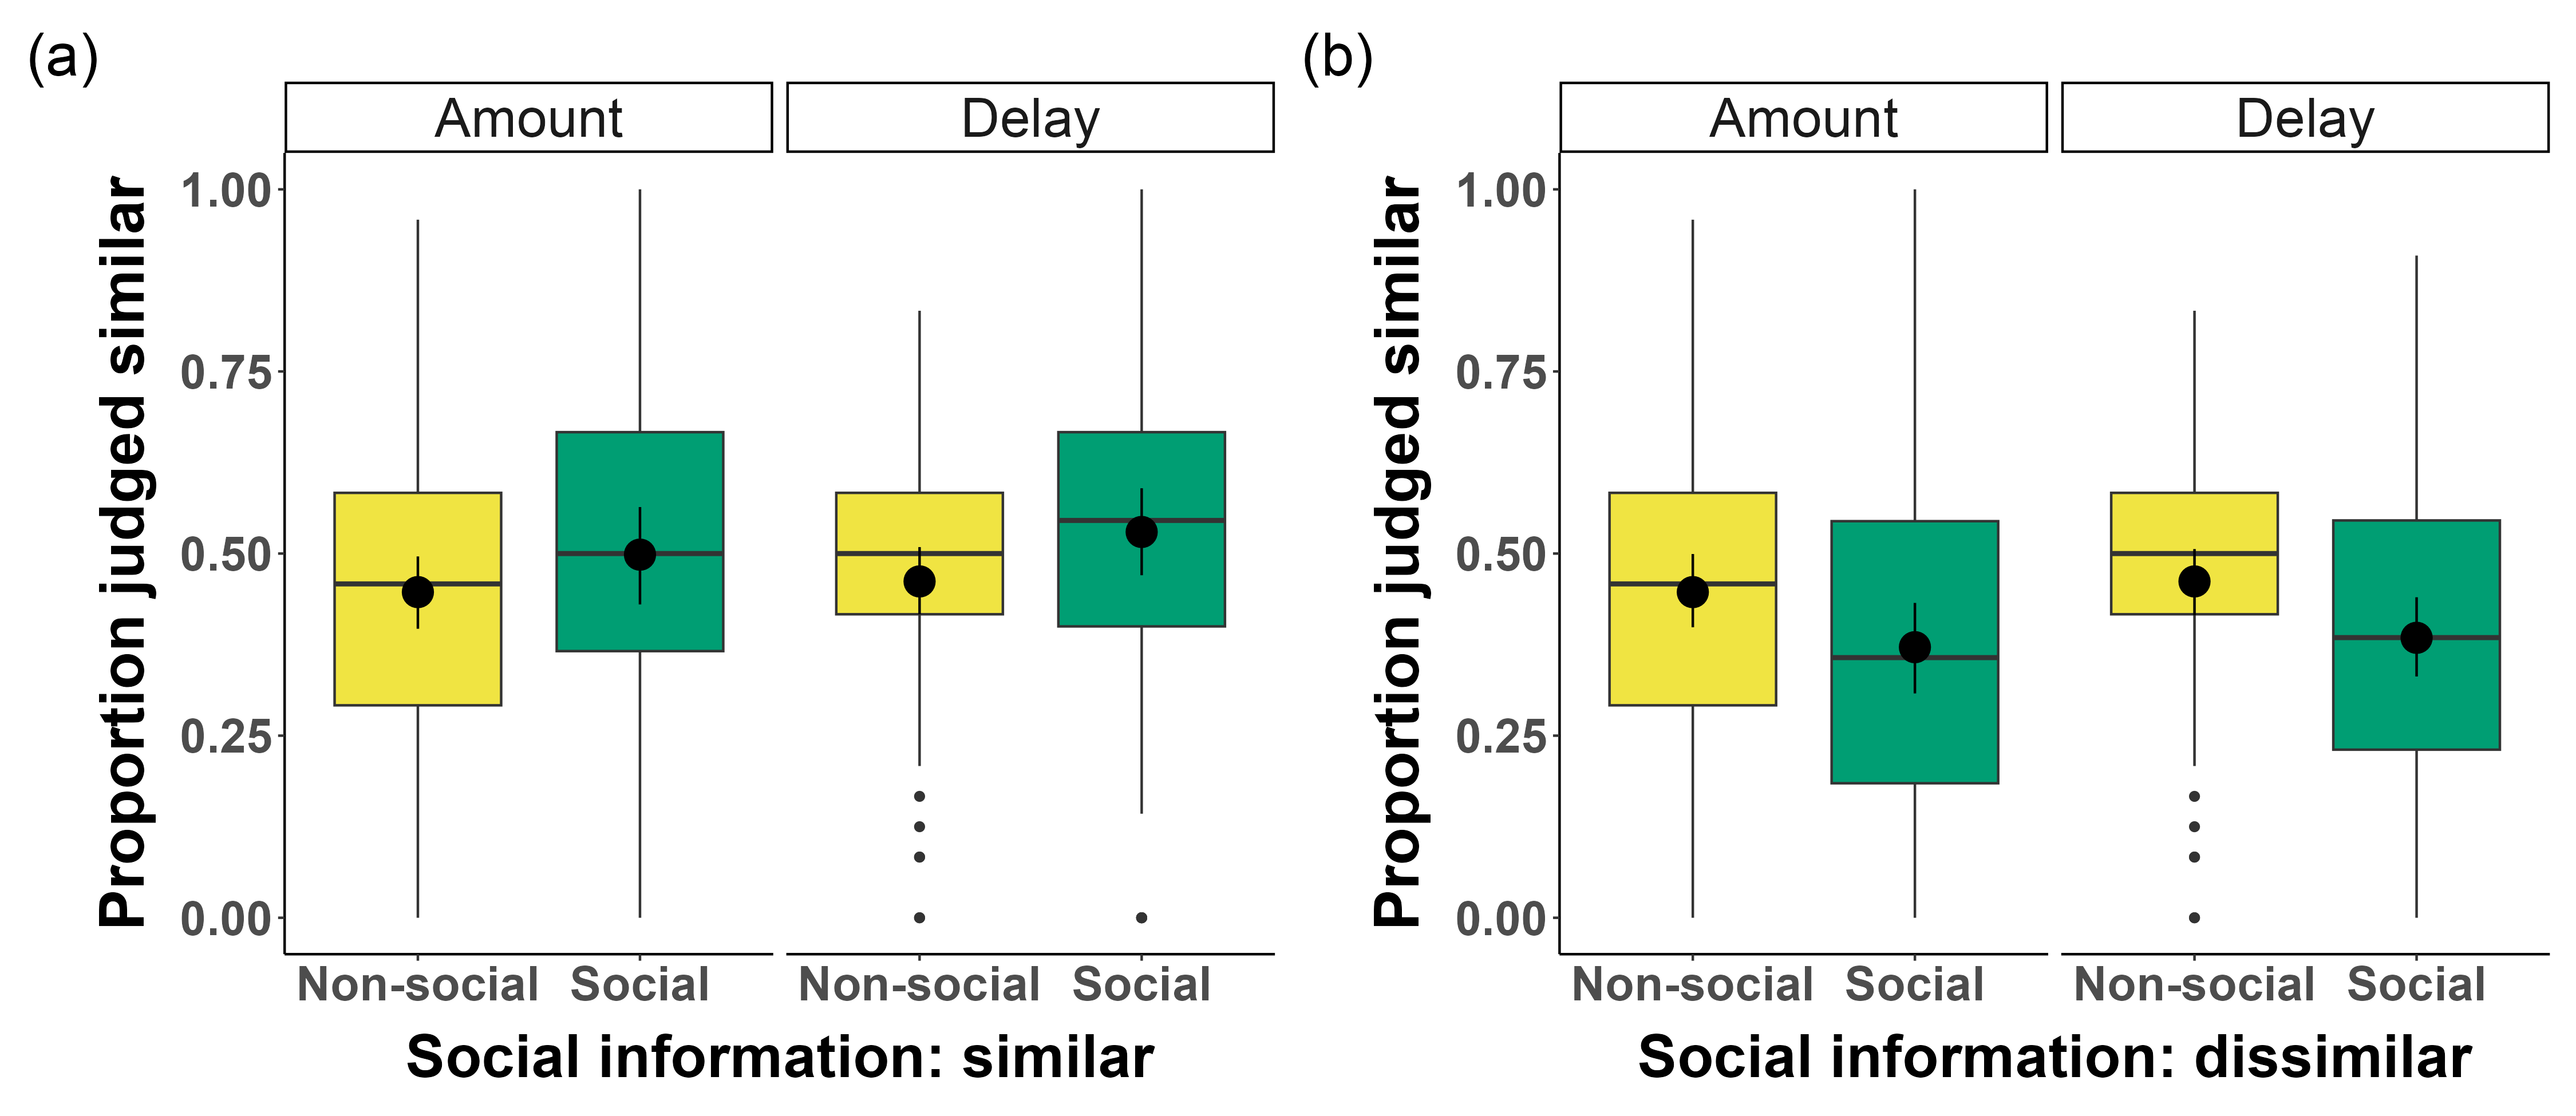
\includegraphics[width=1\linewidth]{figures/judgments_socialinfo_combined_3} \caption{Proportion of number pairs judged similar by participants when the social information suggested that number pairs were (a) similar and (b) dissimilar for Study 3. The left panels represent judgments in the reward amount similarity judgment task while the right panels represent judgments in the time delay similarity judgment task. Dots and error bars represent mean values and 95\% within-subject confidence intervals respectively. For boxplots, horizontal bars represent medians, boxes represent interquartile ranges (25\textsuperscript{th} - 75\textsuperscript{th} percentile), and whiskers represent 1.5 times the interquartile range. Figure used with permission under a CC-BY4.0 license: Goh \& Stevens (2022); available at \url{https://doi.org/10.31234/osf.io/xz68b}}\label{fig:judgmentssocialinfo3}
\end{figure*}

\hypertarget{suggestibility-effects-on-social-influence-2}{%
\subsubsection{Suggestibility effects on social influence}\label{suggestibility-effects-on-social-influence-2}}

To test whether suggestibility moderated the effect of social influence on similarity judgments, we again first categorized participant responses in the social information present condition according to the presented social information (i.e., whether number pairs were suggested to be similar or dissimilar). Participants high in suggestibility were not more influenced by social information in the social version of the similarity judgment tasks compared to participants low in suggestibility when number pairs were either suggested to be similar (\(\chi\)\textsuperscript{2}(2) = 2.20, \emph{p} = .333, \(\mathrm{BF}_{\textrm{10}} < 0.01\)) or dissimilar (\(\chi\)\textsuperscript{2}(2) = 0.83, \emph{p} = .660, \(\mathrm{BF}_{\textrm{10}} < 0.01\); Figure \ref{fig:suggestibility3}).



\begin{figure}

{\centering 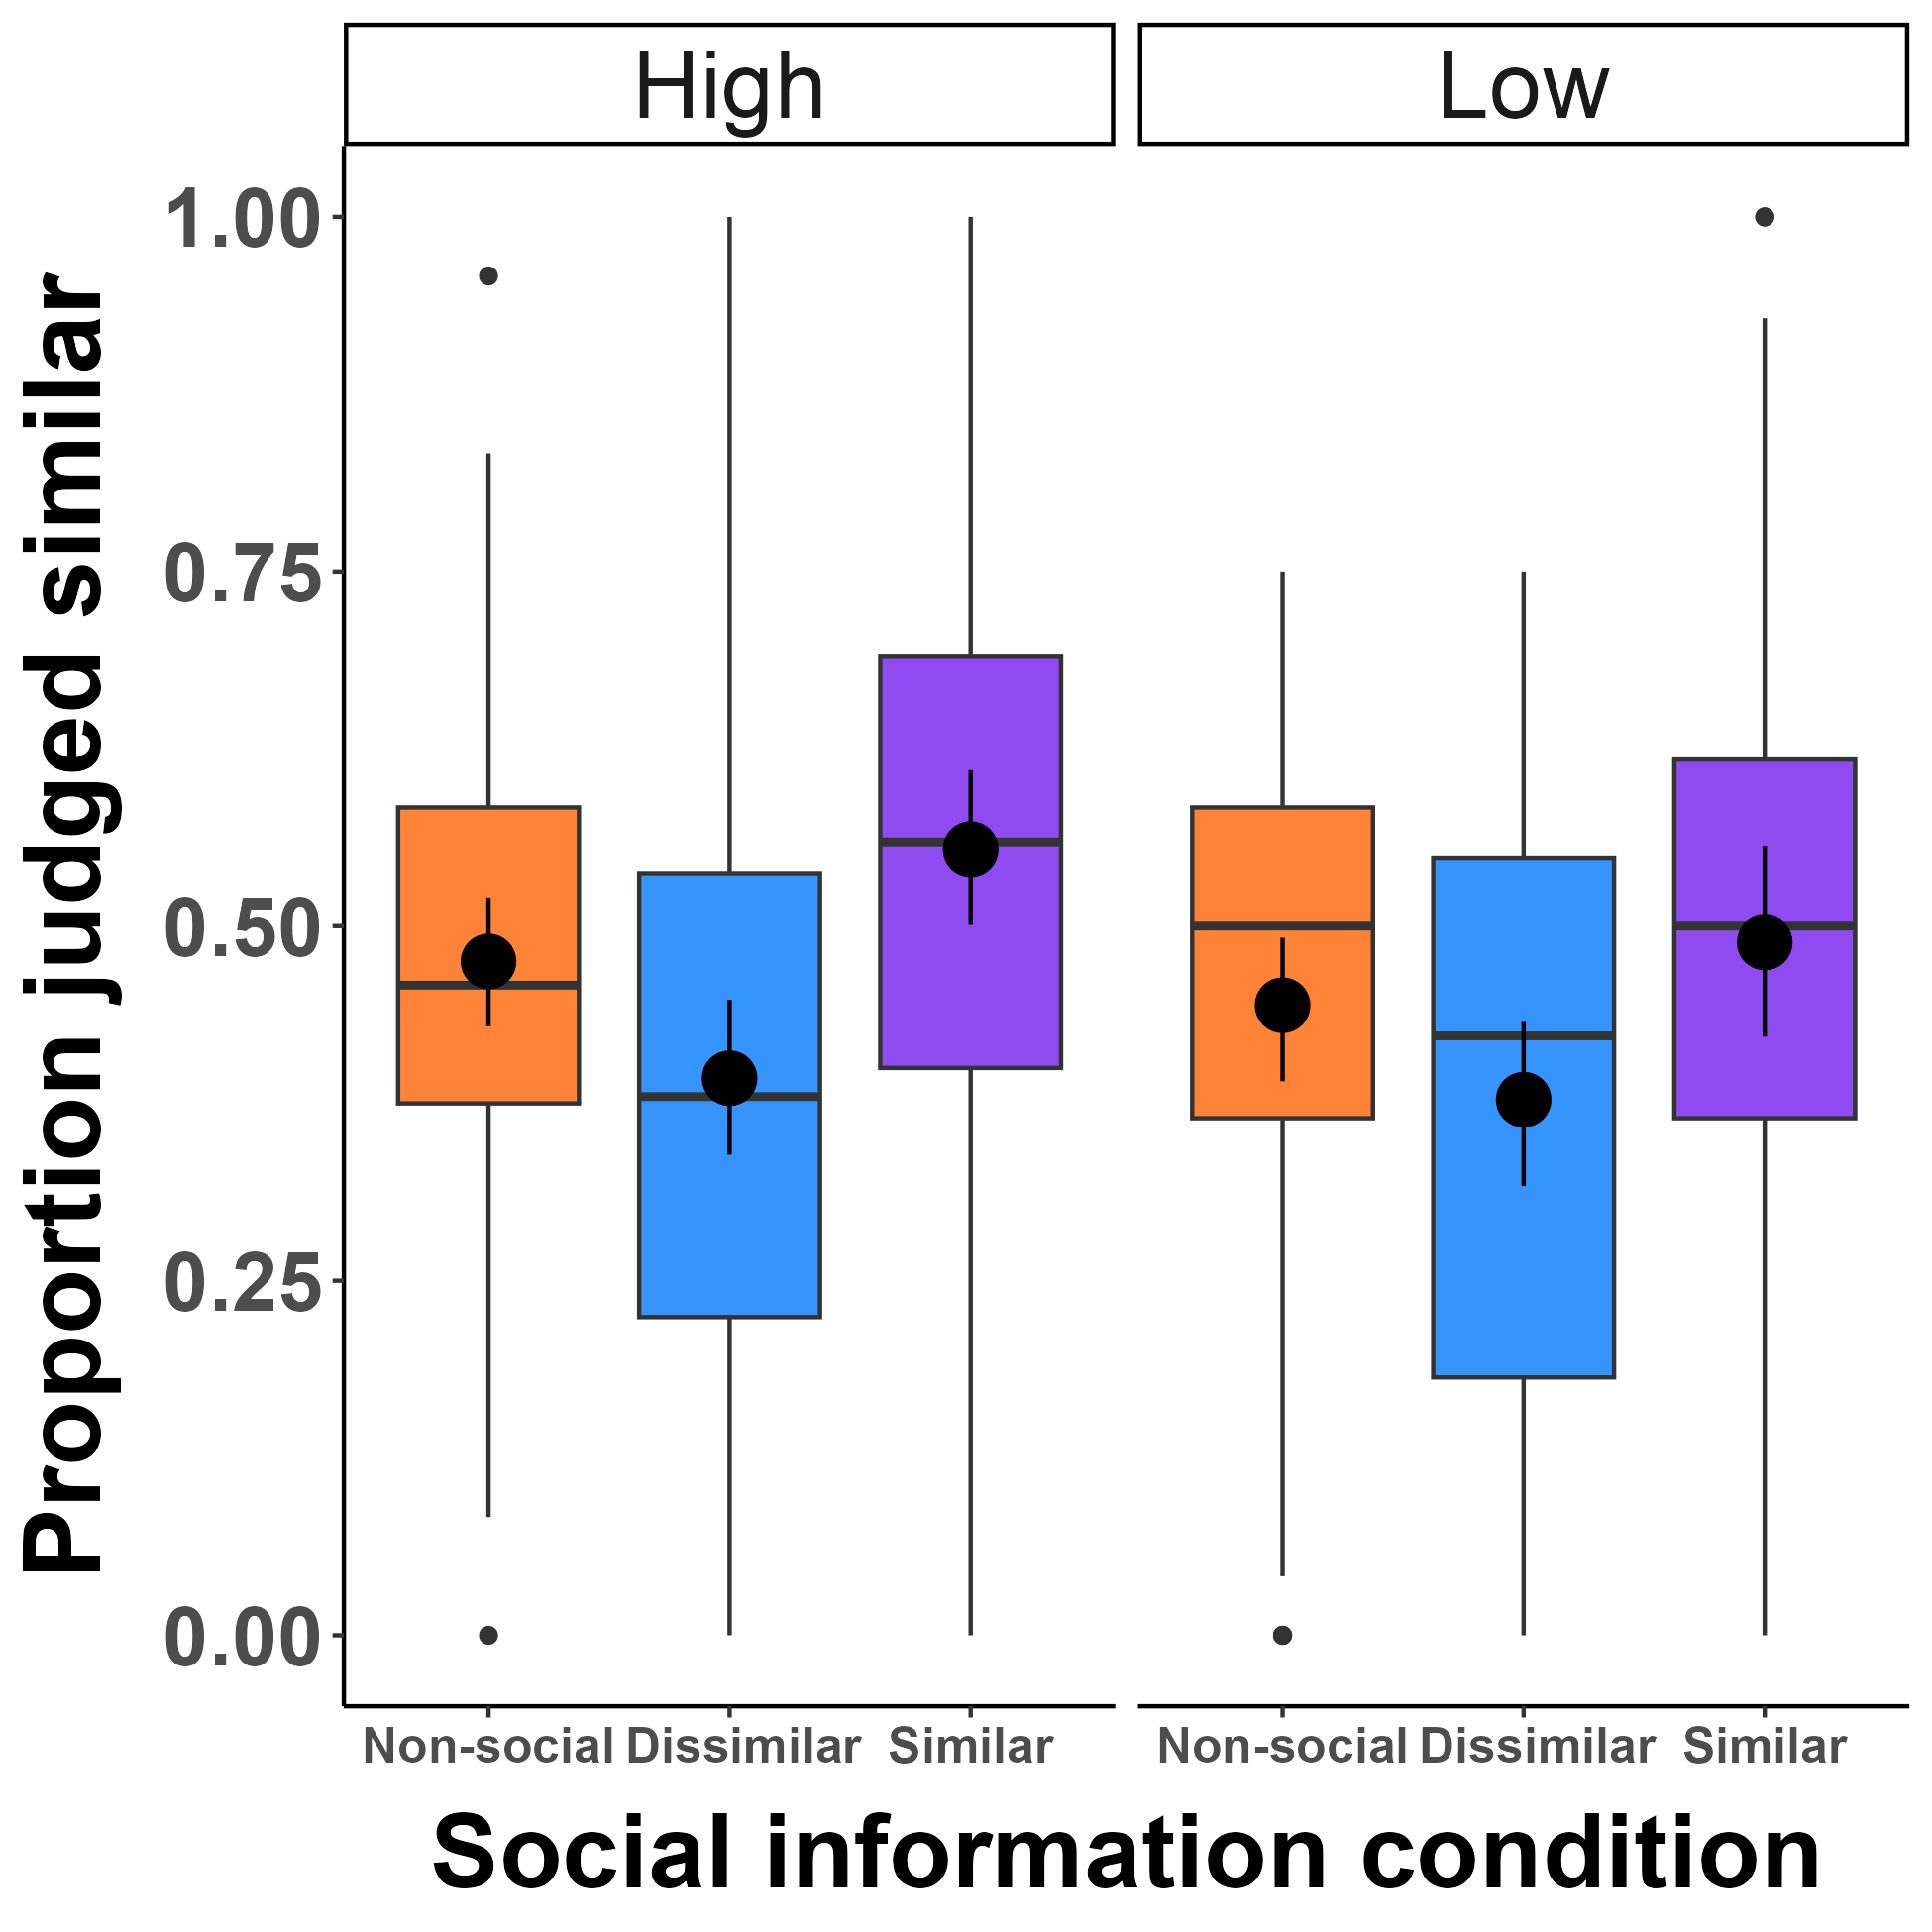
\includegraphics[width=1\linewidth]{figures/suggestibility_social_info_3} 

}

\caption{Proportion of number pairs judged similar by participants for each social information condition for Study 3. The left panel represents similarity judgments for participants in the high suggestibility group while the right panel represents judgments for participants in the low suggestibility group. Dots and error bars represent mean values and 95\% within-subject confidence intervals respectively. For boxplots, horizontal bars represent medians, boxes represent interquartile ranges (25\textsuperscript{th} - 75\textsuperscript{th} percentile), and whiskers represent 1.5 times the interquartile range. Figure used with permission under a CC-BY4.0 license: Goh \& Stevens (2022); available at \url{https://doi.org/10.31234/osf.io/xz68b}}\label{fig:suggestibility3}
\end{figure}

\hypertarget{numeracy-effects-on-similarity-judgments}{%
\subsubsection{Numeracy effects on similarity judgments}\label{numeracy-effects-on-similarity-judgments}}

In terms of objective numeracy, participants with higher objective numeracy scores judged the values in number pairs as more similar compared to participants with lower scores (\(\chi\)\textsuperscript{2}(1) = 13.74, \emph{p} = \textless{} .001, \(\mathrm{BF}_{\textrm{10}} = 12.04\); Figure \ref{fig:numeracyjudgments3}a). Subjective numeracy, however, did not affect similarity judgments for number pairs (\(\chi\)\textsuperscript{2}(1) = 0.01, \emph{p} = .918, \(\mathrm{BF}_{\textrm{10}} = 0.01\); Figure \ref{fig:numeracyjudgments3}b).



\begin{figure*}

{\centering 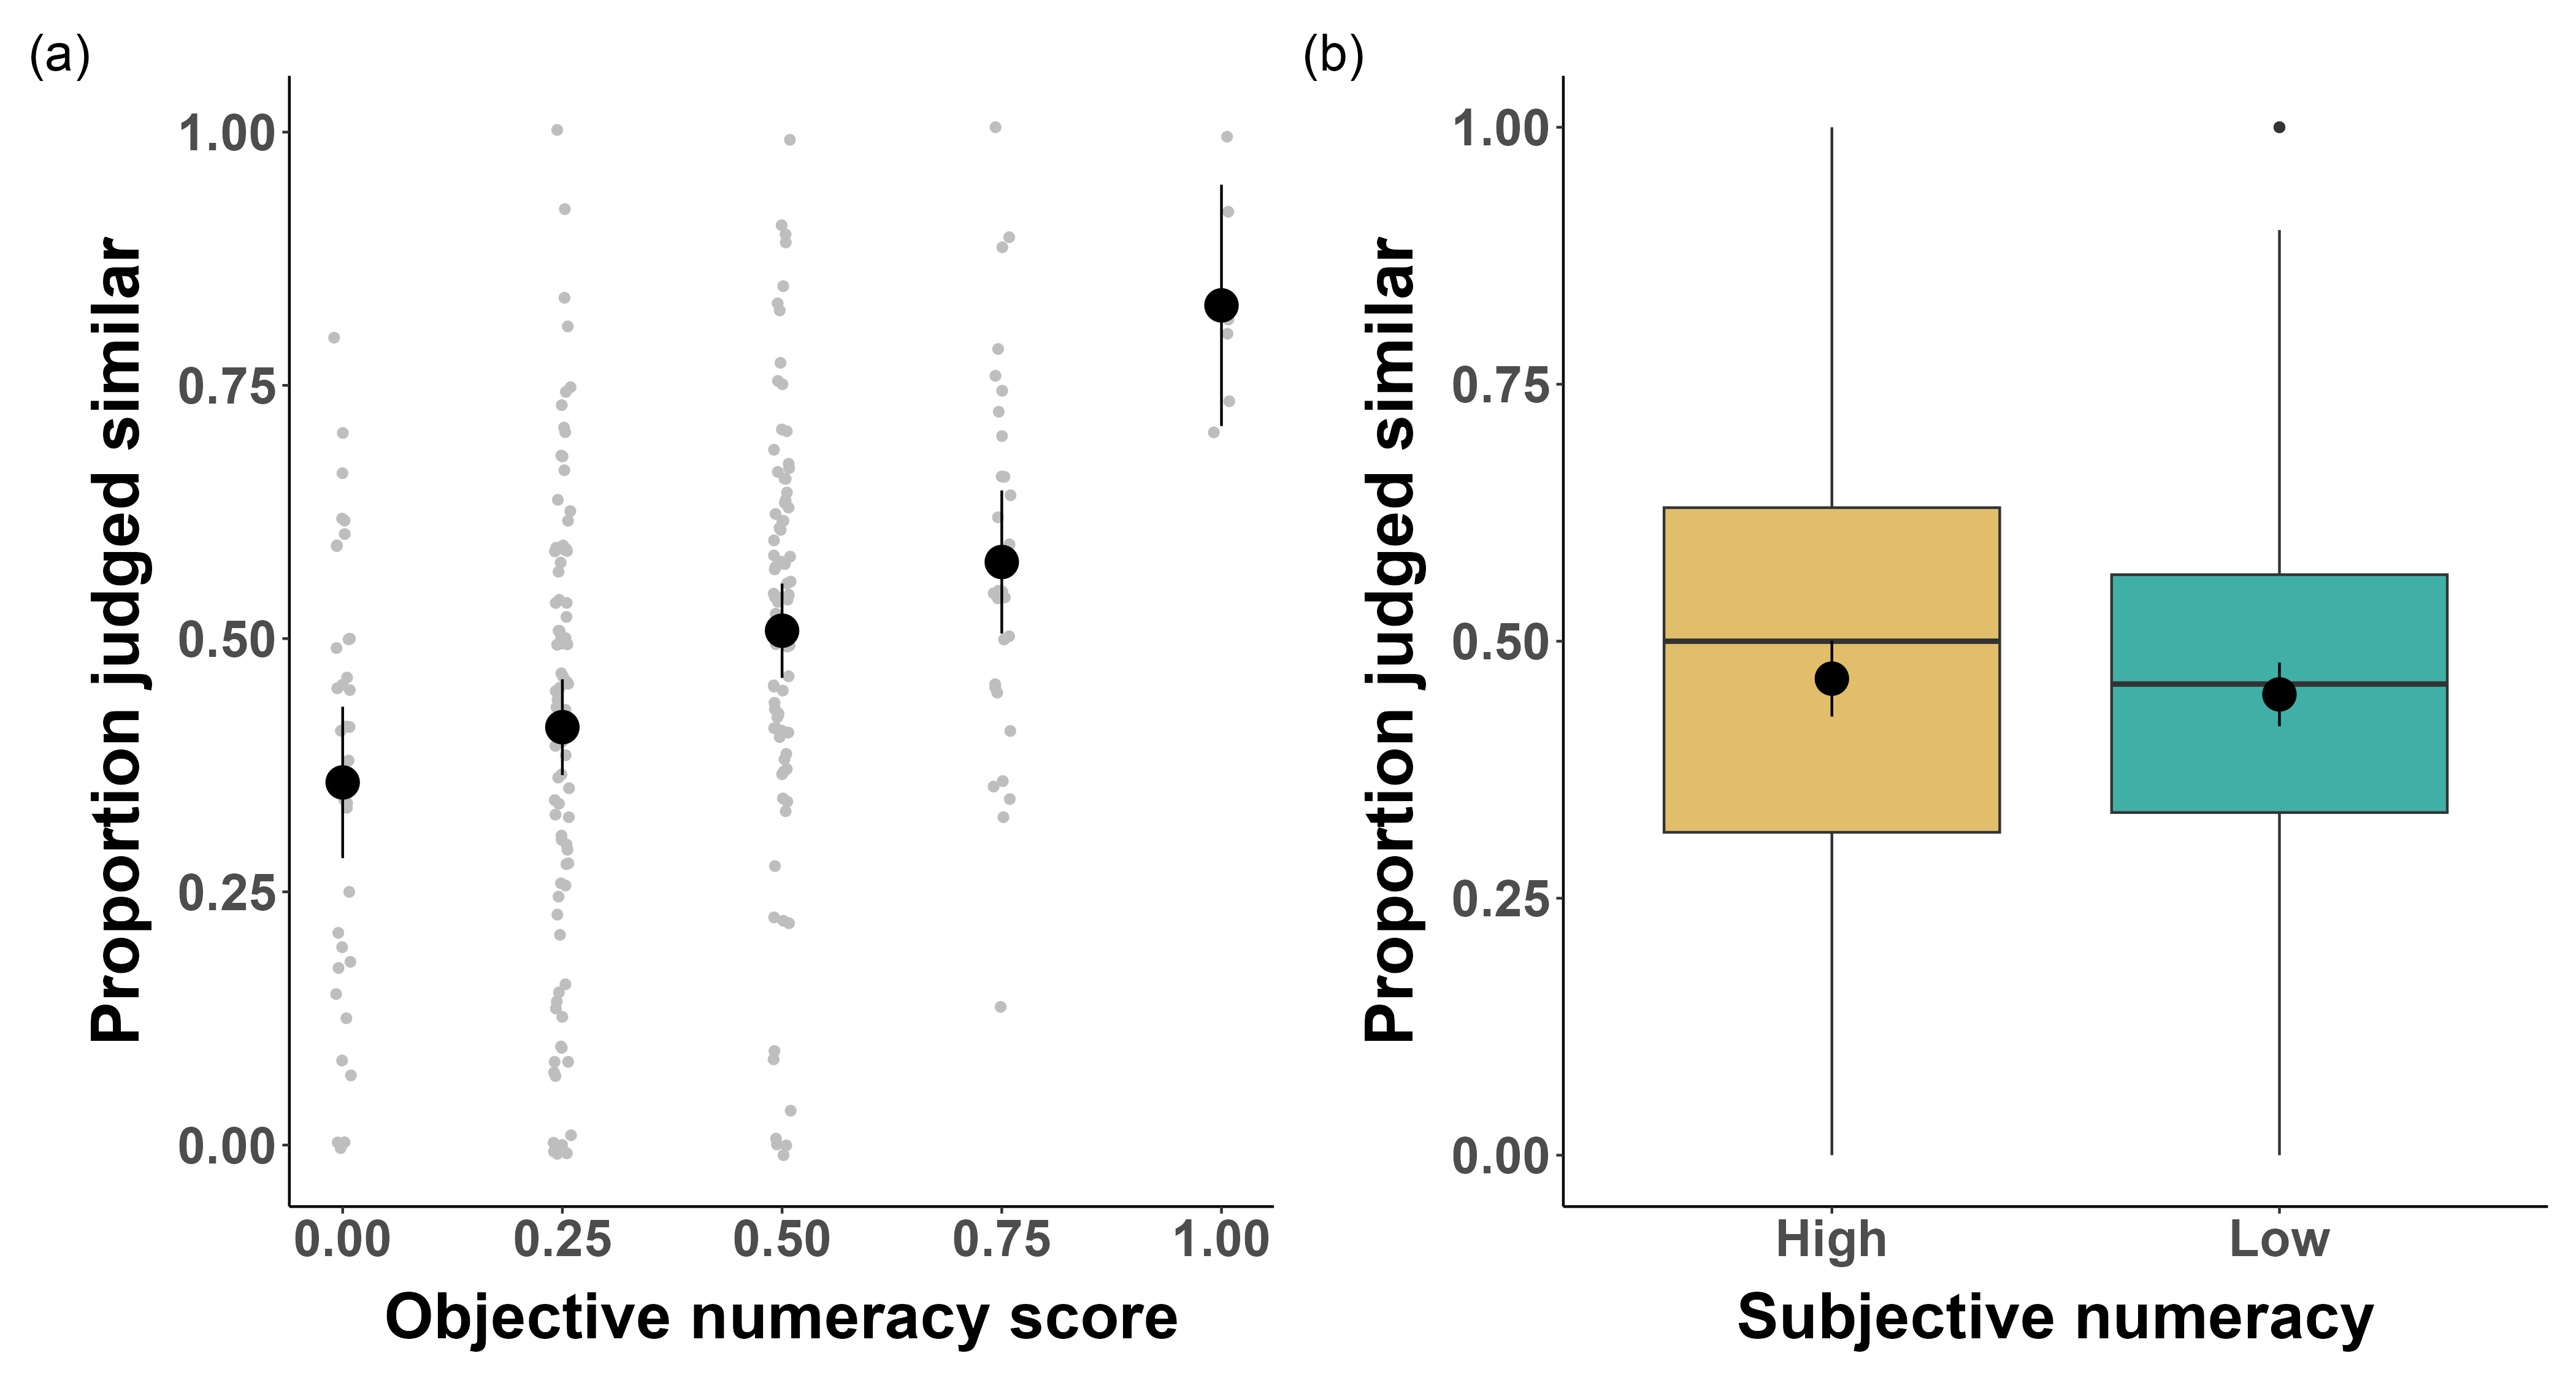
\includegraphics[width=0.8\linewidth]{figures/numeracy_judgments_3} 

}

\caption{Proportion of number pairs judged similar by participants according to (a) objective numeracy scores and (b) subjective numeracy levels for Study 3. Figure used with permission under a CC-BY4.0 license: Goh \& Stevens (2022); available at \url{https://doi.org/10.31234/osf.io/xz68b}}\label{fig:numeracyjudgments3}
\end{figure*}

\hypertarget{discussion-2}{%
\subsection{\texorpdfstring{\emph{Discussion}}{Discussion}}\label{discussion-2}}

The present study aimed to determine if social information about similarity judgments caused people to alter their personal similarity judgments to match the socially suggested ones. Results revealed this to be the case for both judgments of reward amount and time delay number pairs, and that this effect was impervious to individual suggestibility level. Additionally, participants with higher objective numeracy scores tended to judge number pairs to be similar compared to participants with lower numeracy scores. However, finding an overall effect of social information on similarity judgments suggests that social information is powerful enough to shift people's similarity judgments regardless of their numeracy level. The present study thus provides a potential mechanism for the results obtained in Studies 1 and 2.

\hypertarget{general-discussion}{%
\section{General Discussion}\label{general-discussion}}

Receiving social information about other people's similarity judgments for reward amounts and time delays appears to influence personal similarity judgments and subsequent intertemporal choices. Specifically, participant intertemporal choices shifted to match the socially suggested options in the amount-focused condition where they viewed similarity judgments from others that stated reward amounts were dissimilar and time delays were similar. Moreover, participants' personal similarity judgments predicted their non-social intertemporal choices at better than chance level in the amount-focused condition and this finding was echoed when the same social information combination was used to predict participants' choices for social intertemporal choice questions. We found evidence to support that these shifts in intertemporal choices were due to participants changing their similarity judgments to align with the socially suggested similarity judgments. Lastly, individual suggestibility and numeracy did not moderate the effects of social influence on intertemporal choices. While suggestibility did not affect similarity judgments, we found that only participants higher in objective numeracy judged number pairs more similar compared to those with lower objective numeracy.

\hypertarget{implications}{%
\subsection{\texorpdfstring{\emph{Implications}}{Implications}}\label{implications}}

We found that receiving information from others about similarity judgments that promote the larger, later reward can influence one's own decision to choose the larger, later reward. These results support the similarity model of intertemporal choice---the notion that similarity judgments have direct effects on intertemporal choice (Leland, 2002; Rubinstein, 2003; Stevens, 2016). This mechanism of choice predicts that factors that influence similarity judgments can indirectly influence intertemporal choices (Figure \ref{fig:researchframework}). When considered with previous studies that found knowledge of others choosing the larger, later reward can likewise make one choose the larger, later reward (e.g., Kedia et al., 2019; Goto, 2023), our results suggest that the similarity model can serve as an alternative mechanism to traditional discounting models that explain how social information affects intertemporal choice preferences.

Impulsive preferences can detrimentally affect intertemporal decisions ranging from personal finance to environmental sustainability (Hirsh et al., 2015; e.g., Knoll et al., 2015). The ability to shift people's preferences towards the less impulsive option by showing them the similarity judgments of others that promote the larger, later reward could thus potentially help people avoid the temptation of impulsive outcomes and make better intertemporal choices on individual and societal levels. However, waiting for a larger reward may not always be the best choice, especially when visceral factors such as physical hunger threaten the overall well-being of the individual (Loewenstein, 1996) or receipt of the future reward is uncertain (Rick \& Loewenstein, 2008). So, while providing social information may help reduce impulsive choice, this may not be appropriate in all situations.

Finally, our results extend findings on choice preferences to the intertemporal choice domain. We show that people are likely to shift their similarity judgments for amount and delay pairs to match those of others. However, our finding that participants only shifted their intertemporal choices in the amount-focused condition and not in the delay-focused condition suggests that the adoption of a socially suggested option may not be as automatic of a process as suggested by Huh et al. (2014), at least for the domain of intertemporal choice. Thus, those who may want to help others in making better choices for the long term should take note of the extent of the effectiveness of such implicitly established options.

\hypertarget{potential-issues-and-limitations}{%
\subsection{\texorpdfstring{\emph{Potential issues and limitations}}{Potential issues and limitations}}\label{potential-issues-and-limitations}}

Though we found that participants modified their similarity judgments to match those suggested by others, this did not translate to a shift in intertemporal choices in the same manner. Specifically, participants only shifted their intertemporal choices when the socially suggested option was amount-focused. A possible reason why this social influence effect did not occur for the delay-focused condition could be due to the relatively small effect sizes of social information shifting intertemporal choices by 5-6 percentage points. Though social information exerts an influence, the size of the effect is relatively small.

Another reason why people did not choose the smaller, sooner option when they saw delay-focused similarity judgments could be because people show increased future orientation as they reach late adolescence (Steinberg et al., 2009; Göllner et al., 2018). That is, people's propensities to think about their future selves, plan ahead of time, and imagine the consequences of their future actions can lead them to prefer larger, later rewards over smaller, sooner ones. Since our participants were undergraduates whose ages were representative of people in their late adolescence and early adulthood, our results thus align with the notion that people have increased future orientation as they age.

We used monetary amounts as the reward outcome for our intertemporal choice questions. Non-monetary outcomes are discounted more steeply compared to monetary ones (Odum \& Rainaud, 2003; Estle et al., 2007; Odum et al., 2020). However, people who steeply discount for one type of outcome tend to also do so for a variety of outcomes (Odum, 2011; Odum et al., 2020). Based on these findings, it would be interesting to explore whether the social influence effect we found would similarly affect non-monetary outcomes as intertemporal choice contexts can range from choosing what to eat to deciding whether to use substances. Relatedly, we framed our intertemporal choice outcomes as gains that participants could receive. The sign effect posits that people discount gains and losses in intertemporal choice differently, with gains being discounted more heavily than losses regardless of choice domain (Thaler, 1981; Estle et al., 2006, 2007; Hardisty \& Weber, 2009; Hardisty et al., 2013; Stevens, 2016). Thus, future research should explore whether presenting social information that promotes a choice option featuring a loss outcome over another loss option would influence choice like in the present research.

We predicted that suggestibility would moderate the effects of social information on similarity judgments and intertemporal choices based on research that posited suggestibility as a moderating factor of the social influence effect (Gilman et al., 2014). However, we did not find this effect. One reason why we did not find suggestibility effects could be due to differences in analyses; Gilman et al. (2014) calculated discounting scores by taking the difference between the number of smaller, sooner choices that participants made in the condition where they saw others choose the larger, later option and the condition where they saw others choose the smaller, sooner option. In contrast, we calculated the proportion of participants' choices for the larger, later option for each social information condition. Differences in the measurement of intertemporal choice preferences could have thus affected the analysis of suggestibility effects on social influence.

We also predicted that more numerate participants would make fewer similarity judgments in the similarity judgment tasks and prefer the larger, later option in the intertemporal choice task based on work that found highly numerate individuals were less susceptible to option framing effects (Peters, 2012; Ghazal et al., 2014). However, we found that participants higher in objective numeracy made more similarity judgments compared to participants with lower objective numeracy. A possible reason why numeracy did not moderate similarity judgments could be that asking participants to rate monetary amount and time delay pairs on their own did not provide participants with sufficient context to make informed judgments. Providing participants with context for the number pairs they have to make judgments for (e.g., by asking them to imagine themselves receiving one of the two monetary amounts) could thus affect their similarity judgments. Finally, our finding that more numerate participants did not prefer the larger, later intertemporal choice option is in line with research that found either a weak or no relationship between numeracy and preference for the larger, later option in intertemporal choice (Sobkow et al., 2019; Bačová \& Šrol, 2021). This suggests that numeracy effects on intertemporal choice preferences may not be robust across studies and should be examined carefully.

\hypertarget{conclusions}{%
\subsection{\texorpdfstring{\emph{Conclusions}}{Conclusions}}\label{conclusions}}

Decisions seldom occur in silos. People regularly make decisions with social information available, which makes them susceptible to social influence. The present research investigated how observing information about others' similarity judgments affects one's judgments and subsequent intertemporal choices. We showed that people were influenced by others through their similarity judgments to modify their own intertemporal choices when reward outcomes were judged to be different from each other. We also found evidence to support that these shifts in intertemporal choices happened through the mechanism of similarity judgments. Collectively, our results suggest that intertemporal choice preferences can be indirectly established by showing people the similarity judgments of those around them.

\hypertarget{references}{%
\section{References}\label{references}}

\scriptsize

\hypertarget{refs}{}
\begin{CSLReferences}{1}{0}
\leavevmode\vadjust pre{\hypertarget{ref-Bacova.Srol.2021}{}}%
Bačová, V., \& Šrol, J. (2021). Cognitive predictors of delay discounting in monetary choices. \emph{Studia Psychologica}, \emph{63}(2), 129--142. \url{https://doi.org/10.31577/sp.2021.02.817}

\leavevmode\vadjust pre{\hypertarget{ref-Bursztyn.etal.2014}{}}%
Bursztyn, L., Ederer, F., Ferman, B., \& Yuchtman, N. (2014). Understanding mechanisms underlying peer effects: {Evidence} from a field experiment on financial decisions. \emph{Econometrica}, \emph{82}(4), 1273--1301. \url{https://doi.org/10.3982/ECTA11991}

\leavevmode\vadjust pre{\hypertarget{ref-Calluso.etal.2017}{}}%
Calluso, C., Tosoni, A., Fortunato, G., \& Committeri, G. (2017). Can you change my preferences? {Effect} of social influence on intertemporal choice behavior. \emph{Behavioural Brain Research}, \emph{330}, 78--84. \url{https://doi.org/10.1016/j.bbr.2017.05.001}

\leavevmode\vadjust pre{\hypertarget{ref-Cialdini.Goldstein.2004}{}}%
Cialdini, R. B., \& Goldstein, N. J. (2004). Social influence: {Compliance} and conformity. \emph{Annual Review of Psychology}, \emph{55}(1), 591--621. \url{https://doi.org/10.1146/annurev.psych.55.090902.142015}

\leavevmode\vadjust pre{\hypertarget{ref-Cokely.etal.2012}{}}%
Cokely, E. T., Galesic, M., Schulz, E., Garcia-Retamero, R., \& Ghazal, S. (2012). Measuring risk literacy: {The Berlin Numeracy Test}. \emph{Judgment and Decision Making}, \emph{7}(1), 25--47.

\leavevmode\vadjust pre{\hypertarget{ref-Deutsch.Gerard.1955}{}}%
Deutsch, M., \& Gerard, H. B. (1955). A study of normative and informational social influences upon individual judgment. \emph{The Journal of Abnormal and Social Psychology}, \emph{51}(3), 629--636. \url{https://doi.org/10.1037/h0046408}

\leavevmode\vadjust pre{\hypertarget{ref-Doebel.Munakata.2018}{}}%
Doebel, S., \& Munakata, Y. (2018). Group influences on engaging self-control: {Children} delay gratification and value it more when their in-group delays and their out-group doesn't. \emph{Psychological Science}, \emph{29}(5), 738--748. \url{https://doi.org/10.1177/0956797617747367}

\leavevmode\vadjust pre{\hypertarget{ref-Doyle.2013}{}}%
Doyle, J. R. (2013). Survey of time preference, delay discounting models. \emph{Judgment and Decision Making}, \emph{8}(2), 116--135. \url{https://doi.org/10.2139/ssrn.1685861}

\leavevmode\vadjust pre{\hypertarget{ref-Estle.etal.2006}{}}%
Estle, S. J., Green, L., Myerson, J., \& Holt, D. D. (2006). Differential effects of amount on temporal and probability discounting of gains and losses. \emph{Memory \& Cognition}, \emph{34}(4), 914--928. \url{https://doi.org/10.3758/BF03193437}

\leavevmode\vadjust pre{\hypertarget{ref-Estle.etal.2007}{}}%
Estle, S. J., Green, L., Myerson, J., \& Holt, D. D. (2007). Discounting of monetary and directly consumable rewards. \emph{Psychological Science}, \emph{18}(1), 58--63. \url{https://doi.org/10.1111/j.1467-9280.2007.01849.x}

\leavevmode\vadjust pre{\hypertarget{ref-Fagerlin.etal.2007}{}}%
Fagerlin, A., Zikmund-Fisher, B. J., Ubel, P. A., Jankovic, A., Derry, H. A., \& Smith, D. M. (2007). Measuring numeracy without a math test: {Development} of the {Subjective Numeracy Scale}. \emph{Medical Decision Making}, \emph{27}(5), 672--680. \url{https://doi.org/10.1177/0272989X07304449}

\leavevmode\vadjust pre{\hypertarget{ref-Gardner.Steinberg.2005}{}}%
Gardner, M., \& Steinberg, L. (2005). Peer influence on risk taking, risk preference, and risky decision making in adolescence and adulthood: {An} experimental study. \emph{Developmental Psychology}, \emph{41}(4), 625--635. \url{https://doi.org/10.1037/0012-1649.41.4.625}

\leavevmode\vadjust pre{\hypertarget{ref-Ghazal.etal.2014}{}}%
Ghazal, S., Cokely, E. T., \& Garcia-Retamero, R. (2014). Predicting biases in very highly educated samples: {Numeracy} and metacognition. \emph{Judgment and Decision Making}, \emph{9}(1), 15--34.

\leavevmode\vadjust pre{\hypertarget{ref-Gilman.etal.2014}{}}%
Gilman, J. M., Curran, M. T., Calderon, V., Stoeckel, L. E., \& Evins, A. E. (2014). Impulsive social influence increases impulsive choices on a temporal discounting task in young adults. \emph{PLOS ONE}, \emph{9}(7), e101570. \url{https://doi.org/10.1371/journal.pone.0101570}

\leavevmode\vadjust pre{\hypertarget{ref-Goh.Stevens.2021}{}}%
Goh, F. W., \& Stevens, J. R. (2021). Attribute-based choice. In R. Viale (Ed.), \emph{Routledge {Handbook} of {Bounded Rationality}} (pp. 242--253). {Routledge}.

\leavevmode\vadjust pre{\hypertarget{ref-Goldstein.etal.2008}{}}%
Goldstein, N. J., Cialdini, R. B., \& Griskevicius, V. (2008). A room with a viewpoint: {Using} social norms to motivate environmental conservation in hotels. \emph{Journal of Consumer Research}, \emph{35}(3), 472--482. \url{https://doi.org/10.1086/586910}

\leavevmode\vadjust pre{\hypertarget{ref-Gollner.etal.2018}{}}%
Göllner, L. M., Ballhausen, N., Kliegel, M., \& Forstmeier, S. (2018). Delay of gratification, delay discounting and their associations with age, episodic future thinking, and future time perspective. \emph{Frontiers in Psychology}, \emph{8}.

\leavevmode\vadjust pre{\hypertarget{ref-Goto.2023}{}}%
Goto, T. (2023). Normative information can induce biased choice toward delayed larger rewards in adulthood. \emph{Asian Journal of Social Psychology}. \url{https://doi.org/10.1111/ajsp.12562}

\leavevmode\vadjust pre{\hypertarget{ref-Hardisty.etal.2013}{}}%
Hardisty, D. J., Appelt, K. C., \& Weber, E. U. (2013). Good or bad, {We} want it now: {Fixed-cost} present bias for gains and losses explains magnitude asymmetries in intertemporal choice. \emph{Journal of Behavioral Decision Making}, \emph{26}(4), 348--361. \url{https://doi.org/10.1002/bdm.1771}

\leavevmode\vadjust pre{\hypertarget{ref-Hardisty.Weber.2009}{}}%
Hardisty, D. J., \& Weber, E. U. (2009). Discounting future green: {Money} versus the environment. \emph{Journal of Experimental Psychology: General}, \emph{138}(3), 329--340. \url{https://doi.org/10.1037/a0016433}

\leavevmode\vadjust pre{\hypertarget{ref-Hirsh.etal.2015}{}}%
Hirsh, J. L., Costello, M. S., \& Fuqua, R. W. (2015). Analysis of delay discounting as a psychological measure of sustainable behavior. \emph{Behavior and Social Issues}, \emph{24}(1), 187--202. \url{https://doi.org/10.5210/bsi.v24i0.5906}

\leavevmode\vadjust pre{\hypertarget{ref-Huh.etal.2014}{}}%
Huh, Y. E., Vosgerau, J., \& Morewedge, C. K. (2014). Social defaults: {Observed} choices become choice defaults. \emph{Journal of Consumer Research}, \emph{41}(3), 746--760. \url{https://doi.org/10.1086/677315}

\leavevmode\vadjust pre{\hypertarget{ref-Kedia.etal.2019}{}}%
Kedia, G., Brohmer, H., Scholten, M., \& Corcoran, K. (2019). Improving self-control: {The} influence of role models on intertemporal choices. \emph{Frontiers in Psychology}, \emph{10}.

\leavevmode\vadjust pre{\hypertarget{ref-Knoll.etal.2015}{}}%
Knoll, M. A. Z., Appelt, K. C., Johnson, E. J., \& Westfall, J. E. (2015). Time to retire: {Why Americans} claim benefits early \& how to encourage delay. \emph{Behavioral Science \& Policy}, \emph{1}(1), 53--62. \url{https://doi.org/10.1353/bsp.2015.0003}

\leavevmode\vadjust pre{\hypertarget{ref-Kotov.etal.2004}{}}%
Kotov, R. I., Bellman, S. B., \& Watson, D. B. (2004). \emph{Multidimensional {Iowa} suggestibility scale ({MISS})}.

\leavevmode\vadjust pre{\hypertarget{ref-Lee.Chung.2022}{}}%
Lee, H., \& Chung, D. (2022). Characterization of the core determinants of social influence from a computational and cognitive perspective. \emph{Frontiers in Psychiatry}, \emph{13}.

\leavevmode\vadjust pre{\hypertarget{ref-Leland.2002}{}}%
Leland, J. W. (2002). Similarity judgments and anomalies in intertemporal choice. \emph{Economic Inquiry}, \emph{40}(4), 574--581. \url{https://doi.org/10.1093/ei/40.4.574}

\leavevmode\vadjust pre{\hypertarget{ref-R-emmeans}{}}%
Lenth, R. V. (2021). \emph{Emmeans: Estimated marginal means, aka least-squares means}. \url{https://CRAN.R-project.org/package=emmeans}

\leavevmode\vadjust pre{\hypertarget{ref-Loewenstein.1996}{}}%
Loewenstein, G. (1996). Out of control: {Visceral} influences on behavior. \emph{Organizational Behavior and Human Decision Processes}, \emph{65}(3), 272--292. \url{https://doi.org/10.1006/obhd.1996.0028}

\leavevmode\vadjust pre{\hypertarget{ref-Madden.Bickel.2010}{}}%
Madden, G. J., \& Bickel, W. K. (Eds.). (2010). \emph{Impulsivity: The behavioral and neurological science of discounting} (1st ed). {American Psychological Association}.

\leavevmode\vadjust pre{\hypertarget{ref-R-bayestestR}{}}%
Makowski, D., Ben-Shachar, M. S., \& Lüdecke, D. (2019). bayestestR: Describing effects and their uncertainty, existence and significance within the bayesian framework. \emph{Journal of Open Source Software}, \emph{4}(40), 1541. \url{https://doi.org/10.21105/joss.01541}

\leavevmode\vadjust pre{\hypertarget{ref-Mathot.etal.2012}{}}%
Mathôt, S., Schreij, D., \& Theeuwes, J. (2012). {OpenSesame}: {An} open-source, graphical experiment builder for the social sciences. \emph{Behavior Research Methods}, \emph{44}(2), 314--324. \url{https://doi.org/10.3758/s13428-011-0168-7}

\leavevmode\vadjust pre{\hypertarget{ref-R-BayesFactor}{}}%
Morey, R. D., \& Rouder, J. N. (2018). \emph{BayesFactor: Computation of bayes factors for common designs}. \url{https://CRAN.R-project.org/package=BayesFactor}

\leavevmode\vadjust pre{\hypertarget{ref-Morey.etal.2018}{}}%
Morey, R. D., Rouder, J. N., Jamil, T., Urbanek, S., Forner, K., \& Ly, A. (2018). \emph{{BayesFactor}: {Computation} of {Bayes} factors for common designs}.

\leavevmode\vadjust pre{\hypertarget{ref-R-here}{}}%
Müller, K. (2020). \emph{Here: A simpler way to find your files}. \url{https://CRAN.R-project.org/package=here}

\leavevmode\vadjust pre{\hypertarget{ref-Munakata.etal.2020}{}}%
Munakata, Y., Yanaoka, K., Doebel, S., Guild, R. M., Michaelson, L. E., \& Saito, S. (2020). Group influences on children's delay of gratification: {Testing} the roles of culture and personal connections. \emph{Collabra: Psychology}, \emph{6}(1), 1. \url{https://doi.org/10.1525/collabra.265}

\leavevmode\vadjust pre{\hypertarget{ref-R-lsr}{}}%
Navarro, D. (2015). \emph{Learning statistics with r: A tutorial for psychology students and other beginners. (Version 0.6)}. University of New South Wales. \url{https://learningstatisticswithr.com}

\leavevmode\vadjust pre{\hypertarget{ref-OBrien.etal.2011}{}}%
O'Brien, L., Albert, D., Chein, J., \& Steinberg, L. (2011). Adolescents prefer more immediate rewards when in the presence of their peers. \emph{Journal of Research on Adolescence}, \emph{21}(4), 747--753.

\leavevmode\vadjust pre{\hypertarget{ref-Odum.2011}{}}%
Odum, A. L. (2011). Delay discounting: {Trait} variable? \emph{Behavioural Processes}, \emph{87}(1), 1--9. \url{https://doi.org/10.1016/j.beproc.2011.02.007}

\leavevmode\vadjust pre{\hypertarget{ref-Odum.etal.2020}{}}%
Odum, A. L., Becker, R. J., Haynes, J. M., Galizio, A., Frye, C. C. J., Downey, H., Friedel, J. E., \& Perez, D. M. (2020). Delay discounting of different outcomes: {Review} and theory. \emph{Journal of the Experimental Analysis of Behavior}, \emph{113}(3), 657--679. \url{https://doi.org/10.1002/jeab.589}

\leavevmode\vadjust pre{\hypertarget{ref-Odum.Rainaud.2003}{}}%
Odum, A. L., \& Rainaud, C. P. (2003). Discounting of delayed hypothetical money, alcohol, and food. \emph{Behavioural Processes}, \emph{64}(3), 305--313. \url{https://doi.org/10.1016/s0376-6357(03)00145-1}

\leavevmode\vadjust pre{\hypertarget{ref-R-patchwork}{}}%
Pedersen, T. L. (2020). \emph{Patchwork: The composer of plots}. \url{https://CRAN.R-project.org/package=patchwork}

\leavevmode\vadjust pre{\hypertarget{ref-Peters.2012}{}}%
Peters, E. (2012). Beyond comprehension: {The} role of numeracy in judgments and decisions. \emph{Current Directions in Psychological Science}, \emph{21}(1), 31--35. \url{https://doi.org/10.1177/0963721411429960}

\leavevmode\vadjust pre{\hypertarget{ref-R-base}{}}%
R Core Team. (2021). \emph{R: A language and environment for statistical computing}. R Foundation for Statistical Computing. \url{https://www.R-project.org/}

\leavevmode\vadjust pre{\hypertarget{ref-Read.2004}{}}%
Read, D. (2004). Intertemporal choice. In D. J. Koehler \& N. Harvey (Eds.), \emph{Blackwell {Handbook} of {Judgment} and {Decision Making}} (pp. 424--443). {Blackwell}.

\leavevmode\vadjust pre{\hypertarget{ref-Rick.Loewenstein.2008}{}}%
Rick, S., \& Loewenstein, G. (2008). Intangibility in intertemporal choice. \emph{Philosophical Transactions of the Royal Society B: Biological Sciences}, \emph{363}(1511), 3813--3824. \url{https://doi.org/10.1098/rstb.2008.0150}

\leavevmode\vadjust pre{\hypertarget{ref-R-broom}{}}%
Robinson, D., Hayes, A., \& Couch, S. (2021). \emph{Broom: Convert statistical objects into tidy tibbles}. \url{https://CRAN.R-project.org/package=broom}

\leavevmode\vadjust pre{\hypertarget{ref-Rouder.2014}{}}%
Rouder, J. N. (2014). Optional stopping: {No} problem for {Bayesians}. \emph{Psychonomic Bulletin \& Review}, \emph{21}(2), 301--308. \url{https://doi.org/10.3758/s13423-014-0595-4}

\leavevmode\vadjust pre{\hypertarget{ref-Rubinstein.2003}{}}%
Rubinstein, A. (2003). {``{Economics} and psychology''}? {The} case of hyperbolic discounting. \emph{International Economic Review}, \emph{44}(4), 1207--1216.

\leavevmode\vadjust pre{\hypertarget{ref-Schonbrodt.Wagenmakers.2018}{}}%
Schönbrodt, F. D., \& Wagenmakers, E.-J. (2018). Bayes factor design analysis: {Planning} for compelling evidence. \emph{Psychonomic Bulletin \& Review}, \emph{25}(1), 128--142. \url{https://doi.org/10.3758/s13423-017-1230-y}

\leavevmode\vadjust pre{\hypertarget{ref-Schwenke.etal.2022a}{}}%
Schwenke, D., Senftleben, U., \& Scherbaum, S. (2022a). Better together? {Social} distance affects joint probability discounting. \emph{Memory \& Cognition}, \emph{50}(7), 1513--1529. \url{https://doi.org/10.3758/s13421-022-01290-6}

\leavevmode\vadjust pre{\hypertarget{ref-Schwenke.etal.2022}{}}%
Schwenke, D., Wehner, P., \& Scherbaum, S. (2022b). Effects of individual and dyadic decision-making and normative reference on delay discounting decisions. \emph{Cognitive Research: Principles and Implications}, \emph{7}(1), 71. \url{https://doi.org/10.1186/s41235-022-00422-5}

\leavevmode\vadjust pre{\hypertarget{ref-R-afex}{}}%
Singmann, H., Bolker, B., Westfall, J., Aust, F., \& Ben-Shachar, M. S. (2021). \emph{Afex: Analysis of factorial experiments}. \url{https://CRAN.R-project.org/package=afex}

\leavevmode\vadjust pre{\hypertarget{ref-Sobkow.etal.2019}{}}%
Sobkow, A., Fulawka, K., Tomczak, P., Zjawiony, P., \& Traczyk, J. (2019). Does mental number line training work? {The} effects of cognitive training on real-life mathematics, numeracy, and decision making. \emph{Journal of Experimental Psychology: Applied}, \emph{25}(3), 372--385. \url{https://doi.org/10.1037/xap0000207}

\leavevmode\vadjust pre{\hypertarget{ref-Steinberg.etal.2009}{}}%
Steinberg, L., Graham, S., O'Brien, L., Woolard, J., Cauffman, E., \& Banich, M. (2009). Age differences in future orientation and delay discounting. \emph{Child Development}, \emph{80}(1), 28--44. \url{https://doi.org/10.1111/j.1467-8624.2008.01244.x}

\leavevmode\vadjust pre{\hypertarget{ref-Stevens.2016}{}}%
Stevens, J. R. (2016). Intertemporal similarity: {Discounting} as a last resort. \emph{Journal of Behavioral Decision Making}, \emph{29}(1), 12--24. \url{https://doi.org/10.1002/bdm.1870}

\leavevmode\vadjust pre{\hypertarget{ref-Stevens.Soh.2018}{}}%
Stevens, J. R., \& Soh, L.-K. (2018). Predicting similarity judgments in intertemporal choice with machine learning. \emph{Psychonomic Bulletin \& Review}, \emph{25}(2), 627--635. \url{https://doi.org/10.3758/s13423-017-1398-1}

\leavevmode\vadjust pre{\hypertarget{ref-Thaler.1981}{}}%
Thaler, R. (1981). Some empirical evidence on dynamic inconsistency. \emph{Economics Letters}, \emph{8}(3), 201--207. \url{https://doi.org/10.1016/0165-1765(81)90067-7}

\leavevmode\vadjust pre{\hypertarget{ref-Wagenmakers.2007}{}}%
Wagenmakers, E.-J. (2007). A practical solution to the pervasive problems of p values. \emph{Psychonomic Bulletin \& Review}, \emph{14}(5), 779--804. \url{https://doi.org/10.3758/BF03194105}

\leavevmode\vadjust pre{\hypertarget{ref-Wagenmakers.etal.2018}{}}%
Wagenmakers, E.-J., Love, J., Marsman, M., Jamil, T., Ly, A., Verhagen, J., Selker, R., Gronau, Q. F., Dropmann, D., Boutin, B., Meerhoff, F., Knight, P., Raj, A., van Kesteren, E.-J., van Doorn, J., Šmíra, M., Epskamp, S., Etz, A., Matzke, D., \ldots{} Morey, R. D. (2018). Bayesian inference for psychology. {Part II}: {Example} applications with {JASP}. \emph{Psychonomic Bulletin \& Review}, \emph{25}(1), 58--76. \url{https://doi.org/10.3758/s13423-017-1323-7}

\leavevmode\vadjust pre{\hypertarget{ref-Weigard.etal.2014}{}}%
Weigard, A., Chein, J., Albert, D., Smith, A., \& Steinberg, L. (2014). Effects of anonymous peer observation on adolescents' preference for immediate rewards. \emph{Developmental Science}, \emph{17}(1), 71--78. \url{https://doi.org/10.1111/desc.12099}

\leavevmode\vadjust pre{\hypertarget{ref-R-tidyverse}{}}%
Wickham, H., Averick, M., Bryan, J., Chang, W., McGowan, L. D., François, R., Grolemund, G., Hayes, A., Henry, L., Hester, J., Kuhn, M., Pedersen, T. L., Miller, E., Bache, S. M., Müller, K., Ooms, J., Robinson, D., Seidel, D. P., Spinu, V., \ldots{} Yutani, H. (2019). Welcome to the {tidyverse}. \emph{Journal of Open Source Software}, \emph{4}(43), 1686. \url{https://doi.org/10.21105/joss.01686}

\leavevmode\vadjust pre{\hypertarget{ref-Zou.Savani.2019}{}}%
Zou, X., \& Savani, K. (2019). Descriptive norms for me, injunctive norms for you: {Using} norms to explain the risk gap. \emph{Judgment and Decision Making}, \emph{14}(6), 644--648.

\end{CSLReferences}


\end{document}
